\documentclass[11pt,twoside]{book}
\usepackage[utf8]{inputenc}\usepackage[T1]{fontenc}\usepackage{lmodern}
\usepackage{amsmath,amssymb,graphicx,booktabs,array}
\usepackage[margin=1.05in,headheight=14pt]{geometry}
\usepackage{fancyhdr}\pagestyle{fancy}\fancyhf{}
\fancyhead[LE]{\thepage\hfill\textsc{a zoo of topological spaces}}
\fancyhead[RO]{\textsc{\leftmark}\hfill\thepage}\renewcommand{\headrulewidth}{0pt}
\renewcommand{\chaptermark}[1]{\markboth{#1}{}}
\usepackage[hidelinks]{hyperref}
\setlength{\parskip}{3pt}
\newcommand{\entry}[2]{\section{#1}\label{sp:#2}}
\newcommand{\pt}[1]{\par\smallskip\noindent\textit{#1.}\enspace}
\begin{document}
\frontmatter
\begin{titlepage}\centering\vspace*{1.6in}
{\Huge A Zoo of Topological Spaces}\par\vspace{.3in}
{\large Fifty examples with their point-set properties,\\ fundamental groups, homology, derivations, and applications}\par\vfill
{\small Every figure is schematic where a faithful picture is impossible.}\end{titlepage}
\chapter*{Preface}
Courses in topology state general theorems and then say that fundamental groups are hard to compute for most spaces, often without showing why. This collection lists concrete spaces, their invariants, and the reasoning that produces them.

Each entry gives the space, a figure, a table of invariants, a list of point-set properties, and then derivations: first of the point-set properties, then of the fundamental group, homology, and Euler characteristic. Homology is singular homology with integer coefficients, listed as $H_0,H_1,H_2,\dots$; trailing zeros are omitted. The point-set properties of many further spaces can be looked up in the $\pi$-Base database (\texttt{topology.pi-base.org}), which is built on Steen and Seebach's \emph{Counterexamples in Topology}; that database does not record homotopy or homology.

This document is a compilation of standard material, prepared with the assistance of an AI model. None of the definitions, properties, or arguments is original to the compiler. Where a space appears in the $\pi$-Base or in L.~A.~Steen and J.~A.~Seebach, \emph{Counterexamples in Topology}, its entry gives the $\pi$-Base identifier and the example number and page in Steen and Seebach. The standard reference for the algebraic material is A.~Hatcher, \emph{Algebraic Topology}. Full references are at the end.

\tableofcontents
\mainmatter
\chapter{Basic}
\entry{The point}{point}
\noindent$\{*\}$.\enspace One point. Every contractible space is homotopy equivalent to it.
\begin{center}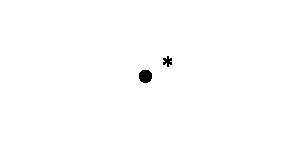
\includegraphics[width=0.5\textwidth,height=2.3in,keepaspectratio]{figs/point.pdf}\end{center}
\begin{center}\renewcommand{\arraystretch}{1.25}\begin{tabular}{>{\raggedleft\arraybackslash}p{.17\textwidth}p{.68\textwidth}}\toprule
$\pi_1$ & $1$\\ $H_*$ & $\mathbb{Z},\ 0,\ 0,\dots$\\ $\chi$ & $1$\\ \midrule
properties & \small compact: yes; connected: yes; path-connected: yes; Hausdorff: yes; manifold: yes; orientable: yes; simply connected: yes; contractible: yes\\ \bottomrule\end{tabular}\end{center}
\pt{Method} Only the constant loop exists.
\pt{Sources} $\pi$-Base \href{https://topology.pi-base.org/spaces/S000162}{S000162}.
\subsection*{Point-set properties}
\pt{Everything}A one-point space is finite, hence compact. Hausdorff holds vacuously. It is $\mathbb{R}^0$, so it is a $0$-manifold.
\subsection*{Algebraic invariants}
\pt{Fundamental group}There is exactly one map $[0,1]\to\{*\}$, so $\pi_1=1$.
\pt{Homology from the definition}There is one singular $n$-simplex $\sigma_n$ in each degree, so $C_n=\mathbb{Z}$. Its boundary is $\partial\sigma_n=\sum_{i=0}^n(-1)^i\sigma_{n-1}$, which is $\sigma_{n-1}$ for $n$ even and $n>0$, and $0$ for $n$ odd. The chain complex is $\cdots\xrightarrow{\ 1\ }\mathbb{Z}\xrightarrow{\ 0\ }\mathbb{Z}\xrightarrow{\ 1\ }\mathbb{Z}\xrightarrow{\ 0\ }\mathbb{Z}\to0$, which is exact except at degree $0$. So $H_0=\mathbb{Z}$ and $H_n=0$ for $n>0$.
\subsection*{Why it is in the zoo}Reference point for contractibility and for the dimension axiom of homology.
\bigskip
\entry{Euclidean space}{rn}
\noindent$\mathbb{R}^n$.\enspace The model space for manifolds.
\begin{center}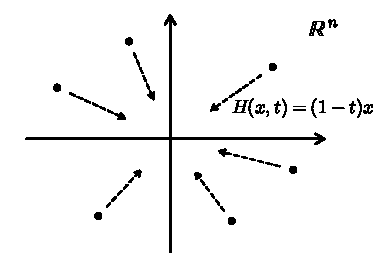
\includegraphics[width=0.5\textwidth,height=2.3in,keepaspectratio]{figs/rn.pdf}\end{center}
\begin{center}\renewcommand{\arraystretch}{1.25}\begin{tabular}{>{\raggedleft\arraybackslash}p{.17\textwidth}p{.68\textwidth}}\toprule
$\pi_1$ & $1$\\ $H_*$ & $\mathbb{Z},\ 0,\ 0,\dots$\\ $\chi$ & $1$\\ \midrule
properties & \small compact: no; connected: yes; path-connected: yes; Hausdorff: yes; manifold: yes; orientable: yes; simply connected: yes; contractible: yes\\ \bottomrule\end{tabular}\end{center}
\pt{Method} Straight-line homotopy to the origin.
\pt{Sources} $\pi$-Base \href{https://topology.pi-base.org/spaces/S000025}{S000025} (the case $n=1$); $\pi$-Base \href{https://topology.pi-base.org/spaces/S000176}{S000176} (the case $n=2$); Steen and Seebach, \emph{Counterexamples in Topology}, Example 28, p.~56.
\subsection*{Point-set properties}
\pt{Not compact}The open balls $B(0,k)$, $k=1,2,\dots$, cover $\mathbb{R}^n$, and any finite subfamily lies in one ball. Equivalently, Heine–Borel fails because $\mathbb{R}^n$ is unbounded.
\pt{Path-connected, Hausdorff}The segment $t\mapsto(1-t)x+ty$ joins $x$ to $y$. Distinct points at distance $d$ have disjoint balls of radius $d/2$.
\pt{Manifold, orientable}The identity is a global chart, and a single chart is an oriented atlas.
\subsection*{Algebraic invariants}
\pt{Contraction}$H(x,t)=(1-t)x$ is continuous with $H_0=\mathrm{id}$ and $H_1$ constant. So $\mathbb{R}^n\simeq\{*\}$ and every homotopy invariant agrees with that of a point.
\subsection*{Why it is in the zoo}Contractible but not compact. Compare the long line, which has trivial homotopy groups yet is not contractible.
\bigskip
\entry{Closed disk}{disk}
\noindent$D^n$.\enspace The unit ball $\{x\in\mathbb{R}^n:|x|\le 1\}$.
\begin{center}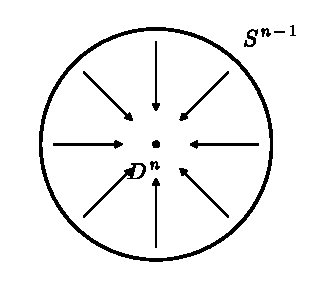
\includegraphics[width=0.5\textwidth,height=2.3in,keepaspectratio]{figs/disk.pdf}\end{center}
\begin{center}\renewcommand{\arraystretch}{1.25}\begin{tabular}{>{\raggedleft\arraybackslash}p{.17\textwidth}p{.68\textwidth}}\toprule
$\pi_1$ & $1$\\ $H_*$ & $\mathbb{Z},\ 0,\dots$\\ $\chi$ & $1$\\ \midrule
properties & \small compact: yes; connected: yes; path-connected: yes; Hausdorff: yes; manifold: with boundary; orientable: yes; simply connected: yes; contractible: yes\\ \bottomrule\end{tabular}\end{center}
\pt{Method} Convex, so straight-line homotopy.
\pt{Sources} Not listed in the $\pi$-Base or in Steen and Seebach.
\subsection*{Point-set properties}
\pt{Compact}Closed and bounded in $\mathbb{R}^n$, so compact by Heine–Borel.
\pt{Manifold with boundary}Interior points have Euclidean balls as neighborhoods. A point with $|x|=1$ has a neighborhood homeomorphic to an open subset of the half-space $\{x_n\ge0\}$, for example via radial coordinates near the boundary sphere.
\subsection*{Algebraic invariants}
\pt{Contraction}$D^n$ is convex, so $H(x,t)=(1-t)x$ stays in $D^n$.
\pt{Brouwer}If $r:D^n\to S^{n-1}$ were a retraction, then $S^{n-1}\hookrightarrow D^n\xrightarrow{r}S^{n-1}$ is the identity. Apply $H_{n-1}$ (with $n\ge2$): the identity of $\mathbb{Z}$ factors through $H_{n-1}(D^n)=0$, a contradiction. A map $f:D^n\to D^n$ without fixed points would give such a retraction by sending $x$ to where the ray from $f(x)$ through $x$ meets the boundary.
\subsection*{Why it is in the zoo}Brouwer's fixed point theorem: $S^{n-1}$ is not a retract of $D^n$, proved with $H_{n-1}$.
\pt{Where it appears} Coverage in sensor networks (\S\ref{app:app-coverage}); Nash equilibrium (\S\ref{app:app-nash}).
\bigskip
\entry{Circle}{circle}
\noindent$S^1$.\enspace The unit circle in $\mathbb{R}^2$, or $\mathbb{R}/\mathbb{Z}$.
\begin{center}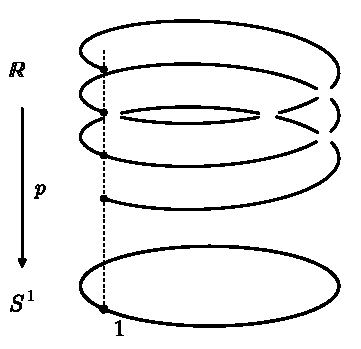
\includegraphics[width=0.5\textwidth,height=2.3in,keepaspectratio]{figs/circle.pdf}\end{center}
\begin{center}\renewcommand{\arraystretch}{1.25}\begin{tabular}{>{\raggedleft\arraybackslash}p{.17\textwidth}p{.68\textwidth}}\toprule
$\pi_1$ & $\mathbb{Z}$\\ $H_*$ & $\mathbb{Z},\ \mathbb{Z},\ 0,\dots$\\ $\chi$ & $0$\\ \midrule
properties & \small compact: yes; connected: yes; path-connected: yes; Hausdorff: yes; manifold: yes; orientable: yes; simply connected: no; contractible: no\\ \bottomrule\end{tabular}\end{center}
\pt{Method} Lift loops through the covering $\mathbb{R}\to S^1$; the endpoint of the lift is the winding number.
\pt{Sources} $\pi$-Base \href{https://topology.pi-base.org/spaces/S000170}{S000170}.
\subsection*{Point-set properties}
\pt{Compact, connected}Closed and bounded in $\mathbb{R}^2$. It is the continuous image of $[0,1]$ under $t\mapsto e^{2\pi it}$, so it is path-connected.
\pt{1-manifold}Removing the point $1$ leaves an open arc homeomorphic to $(0,1)$; removing $-1$ gives a second chart. The transition maps are translations, so the atlas is oriented.
\subsection*{Algebraic invariants}
\pt{Covering}$p:\mathbb{R}\to S^1$, $p(t)=e^{2\pi it}$, is a covering map: each small arc has preimage a disjoint union of intervals, each mapped homeomorphically.
\pt{Degree map}A loop $\gamma$ at $1$ lifts uniquely to $\tilde\gamma$ with $\tilde\gamma(0)=0$, and $\tilde\gamma(1)\in\mathbb{Z}$. Homotopic loops have lifts with the same endpoint (homotopy lifting), so $\deg[\gamma]=\tilde\gamma(1)$ is well defined.
\pt{Isomorphism}Homomorphism: the lift of $\gamma\cdot\delta$ is $\tilde\gamma$ followed by $\tilde\delta+\tilde\gamma(1)$. Surjective: $t\mapsto e^{2\pi int}$ has degree $n$. Injective: if $\tilde\gamma(1)=0$, then $\tilde\gamma$ is a loop in the contractible $\mathbb{R}$; push a null-homotopy down by $p$.
\pt{Homology}CW structure: one $0$-cell $v$, one $1$-cell $a$. Then $\partial a=v-v=0$, so $H_0=H_1=\mathbb{Z}$ and $\chi=1-1=0$.
\subsection*{Why it is in the zoo}The first nontrivial computation. It gives the fundamental theorem of algebra and Brouwer in dimension 2.
\pt{Where it appears} The Aharonov–Bohm effect (\S\ref{app:app-ab}); Topological defects in ordered media (\S\ref{app:app-defects}); A Klein bottle in natural images (\S\ref{app:app-klein}); Grid cells live on a torus (\S\ref{app:app-grid}); Persistent homology and barcodes (\S\ref{app:app-barcodes}); Circular coordinates for periodic data (\S\ref{app:app-circular}); Octave equivalence and the pitch-class circle (\S\ref{app:app-pitchclass}); Meter, polyrhythm, and phasing (\S\ref{app:app-rhythm}); Topological analysis of recorded music (\S\ref{app:app-musicdata}).
\bigskip
\entry{Sphere}{sphere}
\noindent$S^n,\ n\ge 2$.\enspace The unit sphere in $\mathbb{R}^{n+1}$.
\begin{center}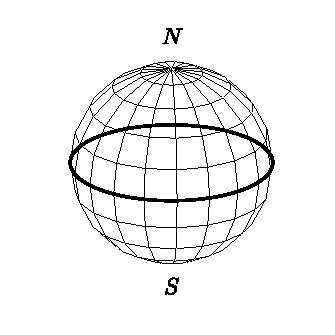
\includegraphics[width=0.5\textwidth,height=2.3in,keepaspectratio]{figs/sphere.pdf}\end{center}
\begin{center}\renewcommand{\arraystretch}{1.25}\begin{tabular}{>{\raggedleft\arraybackslash}p{.17\textwidth}p{.68\textwidth}}\toprule
$\pi_1$ & $1$\\ $H_*$ & $H_0=H_n=\mathbb{Z},\ \text{else }0$\\ $\chi$ & $1+(-1)^n$\\ \midrule
properties & \small compact: yes; connected: yes; path-connected: yes; Hausdorff: yes; manifold: yes; orientable: yes; simply connected: yes; contractible: no\\ \bottomrule\end{tabular}\end{center}
\pt{Method} Van Kampen with two hemispheres whose overlap is path-connected.
\pt{Sources} $\pi$-Base \href{https://topology.pi-base.org/spaces/S000169}{S000169}.
\subsection*{Point-set properties}
\pt{Compact, Hausdorff}Closed and bounded subset of $\mathbb{R}^{n+1}$.
\pt{Path-connected}Two non-antipodal points are joined by the shorter great-circle arc; antipodal points go through any third point.
\pt{Manifold, orientable}Stereographic projection from the north and south poles gives two charts onto $\mathbb{R}^n$. The transition map is inversion $x\mapsto x/|x|^2$ composed with a reflection, and the charts can be chosen so the Jacobian determinant is positive.
\subsection*{Algebraic invariants}
\pt{Fundamental group}Let $U=S^n\setminus\{N\}$ and $V=S^n\setminus\{S\}$. Both are homeomorphic to $\mathbb{R}^n$, and $U\cap V\cong\mathbb{R}^n\setminus\{0\}\simeq S^{n-1}$, which is path-connected for $n\ge2$. Van Kampen gives $\pi_1(S^n)\cong 1*1=1$. For $n=1$ the overlap has two components and the theorem does not apply, which is why $S^1$ is different.
\pt{Homology}CW structure $e^0\cup e^n$. The cellular chain complex is $\mathbb{Z}$ in degrees $0$ and $n$ and zero elsewhere, so every differential vanishes. Alternatively, Mayer–Vietoris with the same $U,V$ gives $\tilde H_k(S^n)\cong\tilde H_{k-1}(S^{n-1})$.
\pt{Euler characteristic}$\chi=1+(-1)^n$: $2$ for even spheres and $0$ for odd ones. Hairy ball: a nowhere-zero vector field on $S^n$ forces $\chi=0$, so even spheres have none.
\pt{Higher homotopy}$\pi_k(S^n)=0$ for $k<n$ (cellular approximation) and $\pi_n(S^n)\cong\mathbb{Z}$ by degree. Above dimension $n$ the groups are hard; see the table at the end.
\subsection*{Why it is in the zoo}Simply connected but not contractible: the first place $\pi_1$ is too weak. $\pi_3(S^2)\cong\mathbb{Z}$ through the Hopf map.
\pt{Where it appears} Spin one-half and the belt trick (\S\ref{app:app-spin}); Topological defects in ordered media (\S\ref{app:app-defects}); The Dirac monopole and charge quantization (\S\ref{app:app-monopole}); Instantons and the vacuum of gauge theory (\S\ref{app:app-instanton}); Qubits, the Bloch sphere, and geometric phase (\S\ref{app:app-bloch}); Persistent homology and barcodes (\S\ref{app:app-barcodes}); Coverage in sensor networks (\S\ref{app:app-coverage}); Orientations, gimbal lock, and quaternions (\S\ref{app:app-attitude}); The hairy ball theorem and the wind (\S\ref{app:app-hairy}); Borsuk–Ulam: antipodes and fair division (\S\ref{app:app-borsuk}).
\bigskip
\entry{Annulus and solid torus}{annulus}
\noindent$S^1\times I,\ \ S^1\times D^2$.\enspace Both deformation retract onto a core circle.
\begin{center}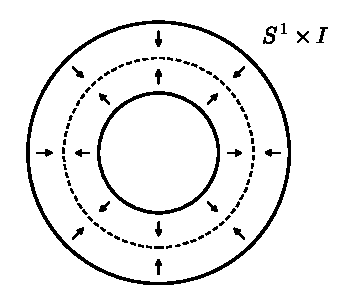
\includegraphics[width=0.5\textwidth,height=2.3in,keepaspectratio]{figs/annulus.pdf}\end{center}
\begin{center}\renewcommand{\arraystretch}{1.25}\begin{tabular}{>{\raggedleft\arraybackslash}p{.17\textwidth}p{.68\textwidth}}\toprule
$\pi_1$ & $\mathbb{Z}$\\ $H_*$ & $\mathbb{Z},\ \mathbb{Z},\ 0,\dots$\\ $\chi$ & $0$\\ \midrule
properties & \small compact: yes; connected: yes; path-connected: yes; Hausdorff: yes; manifold: with boundary; orientable: yes; simply connected: no; contractible: no\\ \bottomrule\end{tabular}\end{center}
\pt{Method} Deformation retract onto $S^1$.
\pt{Sources} Not listed in the $\pi$-Base or in Steen and Seebach.
\subsection*{Point-set properties}
\pt{Compact}Products of compact spaces.
\pt{Manifold with boundary}The annulus is a surface with two boundary circles. The solid torus is a 3-manifold whose boundary is a torus.
\pt{Orientable}Both embed as codimension-zero submanifolds of $\mathbb{R}^2$ and $\mathbb{R}^3$, which are orientable.
\subsection*{Algebraic invariants}
\pt{Deformation retraction}In polar coordinates on $\{1\le r\le2\}$, $H((r,\theta),t)=((1-t)r+t,\theta)$ pushes everything to $r=1$. For $S^1\times D^2$, shrink the disk factor: $(z,w,t)\mapsto(z,(1-t)w)$.
\pt{Invariants}Homotopy equivalent to $S^1$, so $\pi_1=\mathbb{Z}$, $H_1=\mathbb{Z}$, and $\chi=0$.
\subsection*{Why it is in the zoo}$\pi_1$ ignores dimension. The solid torus is half of the genus-one Heegaard splitting of $S^3$ and of every lens space.
\pt{Where it appears} The Aharonov–Bohm effect (\S\ref{app:app-ab}); Chaotic dynamics: the horseshoe and the solenoid (\S\ref{app:app-chaos}).
\bigskip
\entry{Möbius band}{mobius}
\noindent$M$.\enspace $[0,1]\times[0,1]$ with $(0,y)\sim(1,1-y)$.
\begin{center}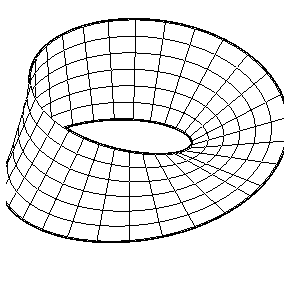
\includegraphics[width=0.5\textwidth,height=2.3in,keepaspectratio]{figs/mobius.pdf}\end{center}
\begin{center}\renewcommand{\arraystretch}{1.25}\begin{tabular}{>{\raggedleft\arraybackslash}p{.17\textwidth}p{.68\textwidth}}\toprule
$\pi_1$ & $\mathbb{Z}$\\ $H_*$ & $\mathbb{Z},\ \mathbb{Z},\ 0$\\ $\chi$ & $0$\\ \midrule
properties & \small compact: yes; connected: yes; path-connected: yes; Hausdorff: yes; manifold: with boundary; orientable: no; simply connected: no; contractible: no\\ \bottomrule\end{tabular}\end{center}
\pt{Method} Retract onto the core circle.
\pt{Sources} Not listed in the $\pi$-Base or in Steen and Seebach.
\subsection*{Point-set properties}
\pt{Compact, Hausdorff}Quotient of a compact square, so compact. It embeds in $\mathbb{R}^3$ by $(\theta,s)\mapsto((1+s\cos\frac\theta2)\cos\theta,(1+s\cos\frac\theta2)\sin\theta,s\sin\frac\theta2)$ with $|s|\le\frac12$, so it is Hausdorff.
\pt{Non-orientable}Carry a small oriented frame once around the core circle $y=\frac12$. The gluing $(0,y)\sim(1,1-y)$ flips the $y$-direction, so the frame returns reflected.
\pt{One boundary circle}The edge $y=0$ is glued at $x=1$ to the start of the edge $y=1$, and vice versa, so the two edges join into a single circle of twice the length.
\subsection*{Algebraic invariants}
\pt{Deformation retraction}$H((x,y),t)=(x,(1-t)y+\frac t2)$. It respects the gluing: $1-y\mapsto(1-t)(1-y)+\frac t2=1-[(1-t)y+\frac t2]$. At $t=1$ everything lies on the core circle.
\pt{The boundary wraps twice}Under the retraction the boundary circle traverses the core twice, so $H_1(\partial M)\to H_1(M)$ is multiplication by $2$. The annulus boundary components map by $\pm1$, which tells the two spaces apart.
\subsection*{Why it is in the zoo}Same homotopy type as the annulus but not homeomorphic: one boundary circle, not two. Gluing a disk to its boundary gives $\mathbb{RP}^2$.
\pt{Where it appears} Two-note chords on a Möbius band (\S\ref{app:app-dyads}); Chord spaces as orbifolds (\S\ref{app:app-orbifold}).
\bigskip
\chapter{Surfaces}
\entry{Torus}{torus}
\noindent$T^2=S^1\times S^1$.\enspace A square with opposite sides identified by the word $aba^{-1}b^{-1}$.
\begin{center}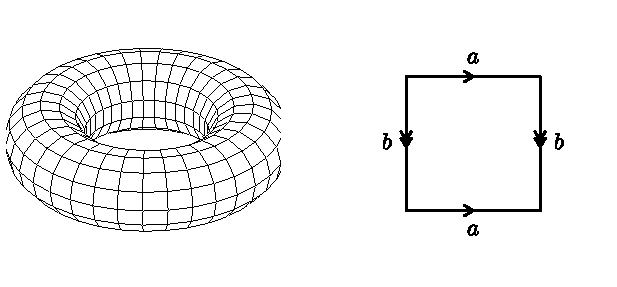
\includegraphics[width=0.82\textwidth,height=2.3in,keepaspectratio]{figs/torus.pdf}\end{center}
\begin{center}\renewcommand{\arraystretch}{1.25}\begin{tabular}{>{\raggedleft\arraybackslash}p{.17\textwidth}p{.68\textwidth}}\toprule
$\pi_1$ & $\mathbb{Z}^2$\\ $H_*$ & $\mathbb{Z},\ \mathbb{Z}^2,\ \mathbb{Z}$\\ $\chi$ & $0$\\ \midrule
properties & \small compact: yes; connected: yes; path-connected: yes; Hausdorff: yes; manifold: yes; orientable: yes; simply connected: no; contractible: no\\ \bottomrule\end{tabular}\end{center}
\pt{Method} $\pi_1(X\times Y)\cong\pi_1X\times\pi_1Y$, or van Kampen on the CW structure.
\pt{Sources} $\pi$-Base \href{https://topology.pi-base.org/spaces/S000224}{S000224}.
\subsection*{Point-set properties}
\pt{Compact, Hausdorff}Product of two compact Hausdorff spaces.
\pt{Manifold, orientable}Products of charts of $S^1$ give charts of $T^2$. In the square model, every edge appears once as $x$ and once as $x^{-1}$, which is the polygon criterion for orientability.
\subsection*{Algebraic invariants}
\pt{Fundamental group}A loop in $X\times Y$ is a pair of loops, and homotopies act coordinatewise, so $\pi_1(T^2)\cong\mathbb{Z}\times\mathbb{Z}$. In the square, the relation $aba^{-1}b^{-1}=1$ is the boundary of the 2-cell.
\pt{Cellular homology}One $0$-cell $v$, $1$-cells $a,b$, one $2$-cell $e$. Then $\partial a=\partial b=v-v=0$ and $\partial e=a+b-a-b=0$. All differentials vanish, so $H=\mathbb{Z},\mathbb{Z}^2,\mathbb{Z}$ and $\chi=1-2+1=0$.
\pt{Universal cover}$\mathbb{R}^2\to\mathbb{R}^2/\mathbb{Z}^2$. Since $\mathbb{R}^2$ is contractible, $T^2$ is aspherical: $\pi_k(T^2)=0$ for $k\ge2$.
\subsection*{Why it is in the zoo}The universal cover $\mathbb{R}^2$ with deck group $\mathbb{Z}^2$ is the cleanest example of the covering correspondence.
\pt{Where it appears} The quantum Hall effect and Chern numbers (\S\ref{app:app-hall}); The toric code (\S\ref{app:app-toric}); Grid cells live on a torus (\S\ref{app:app-grid}); Two-note chords on a Möbius band (\S\ref{app:app-dyads}); The Tonnetz is a torus (\S\ref{app:app-tonnetz}); Meter, polyrhythm, and phasing (\S\ref{app:app-rhythm}); Topological analysis of recorded music (\S\ref{app:app-musicdata}); The hairy ball theorem and the wind (\S\ref{app:app-hairy}).
\bigskip
\entry{n-torus}{ntorus}
\noindent$T^n$.\enspace Product of $n$ circles; $\mathbb{R}^n/\mathbb{Z}^n$.
\begin{center}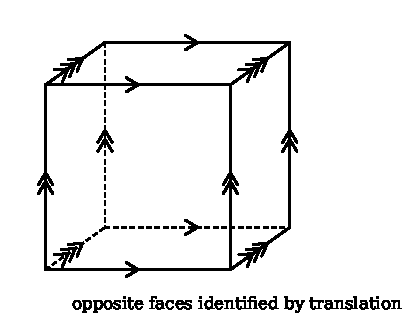
\includegraphics[width=0.5\textwidth,height=2.3in,keepaspectratio]{figs/ntorus.pdf}\end{center}
\begin{center}\renewcommand{\arraystretch}{1.25}\begin{tabular}{>{\raggedleft\arraybackslash}p{.17\textwidth}p{.68\textwidth}}\toprule
$\pi_1$ & $\mathbb{Z}^n$\\ $H_*$ & $H_k\cong \mathbb{Z}^{\binom nk}$\\ $\chi$ & $0$\\ \midrule
properties & \small compact: yes; connected: yes; path-connected: yes; Hausdorff: yes; manifold: yes; orientable: yes; simply connected: no; contractible: no\\ \bottomrule\end{tabular}\end{center}
\pt{Method} Product formula; homology from the product cell structure.
\pt{Sources} Not listed in the $\pi$-Base or in Steen and Seebach.
\subsection*{Point-set properties}
\pt{Compact, manifold, orientable}Finite product of compact orientable manifolds. The cube $[0,1]^n$ with opposite faces glued by translations is another model.
\subsection*{Algebraic invariants}
\pt{Fundamental group}Product formula, or the covering $\mathbb{R}^n\to T^n$ with deck group $\mathbb{Z}^n$.
\pt{Homology}The product CW structure has one $k$-cell for each $k$-element subset of the $n$ coordinates, so $\binom nk$ cells in degree $k$. Each circle factor has zero differential, and the product differential is built from these, so it vanishes. Hence $H_k\cong\mathbb{Z}^{\binom nk}$.
\pt{Euler characteristic}$\chi=\sum_k(-1)^k\binom nk=(1-1)^n=0$.
\subsection*{Why it is in the zoo}$T^n$ is a $K(\mathbb{Z}^n,1)$. The binomial Betti numbers are a good Künneth exercise.
\pt{Where it appears} The quantum Hall effect and Chern numbers (\S\ref{app:app-hall}); The shape of the universe (\S\ref{app:app-cosmic}); Chord spaces as orbifolds (\S\ref{app:app-orbifold}); Robot arms and motion planning (\S\ref{app:app-robots}).
\bigskip
\entry{Orientable surface of genus g}{genusg}
\noindent$\Sigma_g,\ g\ge 1$.\enspace Connected sum of $g$ tori; a $4g$-gon with word $a_1b_1a_1^{-1}b_1^{-1}\cdots a_gb_ga_g^{-1}b_g^{-1}$.
\begin{center}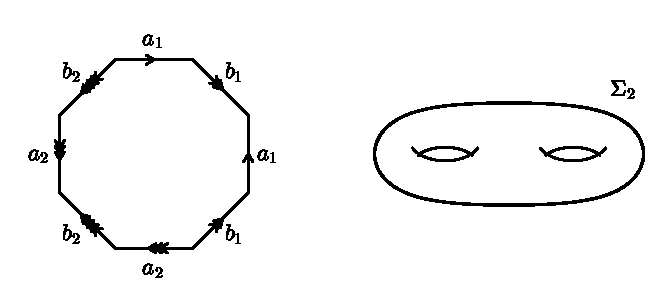
\includegraphics[width=0.82\textwidth,height=2.3in,keepaspectratio]{figs/genusg.pdf}\end{center}
\begin{center}\renewcommand{\arraystretch}{1.25}\begin{tabular}{>{\raggedleft\arraybackslash}p{.17\textwidth}p{.68\textwidth}}\toprule
$\pi_1$ & $\langle a_1,b_1,\dots,a_g,b_g \mid [a_1,b_1]\cdots[a_g,b_g]\rangle$\\ $H_*$ & $\mathbb{Z},\ \mathbb{Z}^{2g},\ \mathbb{Z}$\\ $\chi$ & $2-2g$\\ \midrule
properties & \small compact: yes; connected: yes; path-connected: yes; Hausdorff: yes; manifold: yes; orientable: yes; simply connected: no; contractible: no\\ \bottomrule\end{tabular}\end{center}
\pt{Method} Van Kampen: the 1-skeleton is a wedge of 2g circles and the 2-cell adds one relation.
\pt{Sources} Not listed in the $\pi$-Base or in Steen and Seebach.
\subsection*{Point-set properties}
\pt{Compact, Hausdorff}Quotient of a compact polygon. It embeds in $\mathbb{R}^3$ as the surface of a $g$-holed doughnut, so it is Hausdorff.
\pt{2-manifold}Interior points of the polygon have disk neighborhoods. An edge point gets two half-disks glued along a diameter. All $4g$ vertices go to one point, and their $4g$ corner sectors fit together around it into a full disk.
\pt{Orientable}Each edge label appears once with exponent $+1$ and once with $-1$, so the gluings reverse the boundary direction and the polygon's orientation extends across every edge.
\subsection*{Algebraic invariants}
\pt{Van Kampen}Let $U$ be the open 2-cell and $V$ the complement of its center. $U$ is contractible, $V$ deformation retracts onto the 1-skeleton (a wedge of $2g$ circles, so $\pi_1(V)=F_{2g}$), and $U\cap V$ is an annulus whose generator maps to the boundary word. So $\pi_1=F_{2g}/\langle\langle[a_1,b_1]\cdots[a_g,b_g]\rangle\rangle$.
\pt{Cellular homology}One $0$-cell, $2g$ $1$-cells, one $2$-cell. The boundary of the 2-cell is $\sum_i(a_i+b_i-a_i-b_i)=0$, and the $1$-cells are loops. All differentials vanish.
\pt{Euler characteristic}$\chi=1-2g+1=2-2g$. Since $H_1=\mathbb{Z}^{2g}$ determines $g$, different genera give non-homeomorphic surfaces.
\subsection*{Why it is in the zoo}For $g\ge2$ the group is non-abelian and hyperbolic. $H_1=\mathbb{Z}^{2g}$ is its abelianization, a concrete case of Hurewicz.
\pt{Where it appears} The toric code (\S\ref{app:app-toric}).
\bigskip
\entry{Real projective plane}{rp2}
\noindent$\mathbb{RP}^2$.\enspace $S^2$ with antipodal points identified; a disk with antipodal boundary points identified.
\begin{center}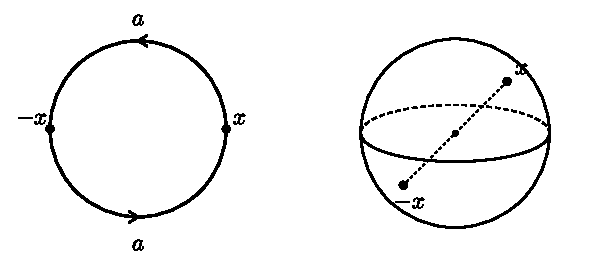
\includegraphics[width=0.82\textwidth,height=2.3in,keepaspectratio]{figs/rp2.pdf}\end{center}
\begin{center}\renewcommand{\arraystretch}{1.25}\begin{tabular}{>{\raggedleft\arraybackslash}p{.17\textwidth}p{.68\textwidth}}\toprule
$\pi_1$ & $\mathbb{Z}/2$\\ $H_*$ & $\mathbb{Z},\ \mathbb{Z}/2,\ 0$\\ $\chi$ & $1$\\ \midrule
properties & \small compact: yes; connected: yes; path-connected: yes; Hausdorff: yes; manifold: yes; orientable: no; simply connected: no; contractible: no\\ \bottomrule\end{tabular}\end{center}
\pt{Method} Two-sheeted universal cover $S^2\to\mathbb{RP}^2$.
\pt{Sources} $\pi$-Base \href{https://topology.pi-base.org/spaces/S000168}{S000168}.
\subsection*{Point-set properties}
\pt{Compact}Continuous image of $S^2$.
\pt{Hausdorff}If $[x]\ne[y]$, choose $\varepsilon$ smaller than the distances between $\pm x$ and $\pm y$. The images of the four $\varepsilon$-balls around $\pm x,\pm y$ are disjoint open sets.
\pt{2-manifold}A small cap on $S^2$ contains no antipodal pair, so it maps homeomorphically onto its image.
\pt{Non-orientable}A neighborhood of a projective line (the image of a great circle) is a Möbius band.
\subsection*{Algebraic invariants}
\pt{Fundamental group}$p:S^2\to\mathbb{RP}^2$ is a covering with deck group $\{\pm1\}$. $S^2$ is simply connected, so it is the universal cover and $\pi_1\cong\mathbb{Z}/2$. The generator is the image of a path from a point to its antipode.
\pt{Cellular homology}Cells $e^0,e^1,e^2$, with $e^2$ attached along the word $aa$. The chain complex is $0\to\mathbb{Z}\xrightarrow{\ 2\ }\mathbb{Z}\xrightarrow{\ 0\ }\mathbb{Z}\to0$. So $H_0=\mathbb{Z}$, $H_1=\mathbb{Z}/2$, and $H_2=\ker(\times2)=0$.
\pt{Euler characteristic}$\chi=1-1+1=1$, consistent with $\chi(S^2)=2\chi(\mathbb{RP}^2)$ for a 2-sheeted cover.
\subsection*{Why it is in the zoo}The smallest nontrivial finite fundamental group and the first torsion in homology. It does not embed in $\mathbb{R}^3$.
\pt{Where it appears} Topological defects in ordered media (\S\ref{app:app-defects}).
\bigskip
\entry{Klein bottle}{klein}
\noindent$K$.\enspace A square with word $abab^{-1}$; two Möbius bands glued along their boundaries.
\begin{center}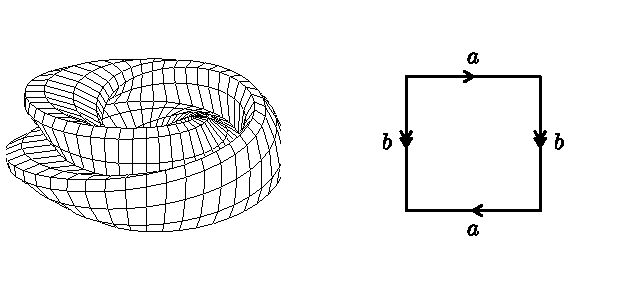
\includegraphics[width=0.82\textwidth,height=2.3in,keepaspectratio]{figs/klein.pdf}\end{center}
\begin{center}\renewcommand{\arraystretch}{1.25}\begin{tabular}{>{\raggedleft\arraybackslash}p{.17\textwidth}p{.68\textwidth}}\toprule
$\pi_1$ & $\langle a,b\mid abab^{-1}\rangle$\\ $H_*$ & $\mathbb{Z},\ \mathbb{Z}\oplus\mathbb{Z}/2,\ 0$\\ $\chi$ & $0$\\ \midrule
properties & \small compact: yes; connected: yes; path-connected: yes; Hausdorff: yes; manifold: yes; orientable: no; simply connected: no; contractible: no\\ \bottomrule\end{tabular}\end{center}
\pt{Method} Van Kampen on the square, then abelianize.
\pt{Sources} Not listed in the $\pi$-Base or in Steen and Seebach.
\subsection*{Point-set properties}
\pt{Compact, Hausdorff}Quotient of a square; it embeds in $\mathbb{R}^4$, so it is Hausdorff. In $\mathbb{R}^3$ it can only be immersed.
\pt{2-manifold, non-orientable}The polygon argument gives a manifold. The edge $a$ appears twice with the same exponent, so a strip across it is a Möbius band.
\subsection*{Algebraic invariants}
\pt{Fundamental group}One vertex, edges $a,b$, and a 2-cell attached along $abab^{-1}$. Van Kampen gives $\langle a,b\mid abab^{-1}\rangle$, equivalently $bab^{-1}=a^{-1}$.
\pt{Non-abelian}$\pi_1$ is torsion-free (the universal cover is $\mathbb{R}^2$), so $a\ne a^{-1}$, and $bab^{-1}=a^{-1}\ne a$.
\pt{Torus double cover}$b^2ab^{-2}=ba^{-1}b^{-1}=a$, so $a$ and $b^2$ commute. The subgroup $\langle a,b^2\rangle\cong\mathbb{Z}^2$ has index $2$ and corresponds to a torus double cover.
\pt{Cellular homology}$\partial a=\partial b=0$ and $\partial e=a+b+a-b=2a$. So $H_1=\mathbb{Z}\langle a,b\rangle/\langle 2a\rangle=\mathbb{Z}\oplus\mathbb{Z}/2$ and $H_2=\ker\partial_2=0$. $\chi=1-2+1=0$.
\subsection*{Why it is in the zoo}Same Euler characteristic as the torus; homology tells them apart. $\pi_1$ is non-abelian but contains $\mathbb{Z}^2$ with index 2.
\pt{Where it appears} A Klein bottle in natural images (\S\ref{app:app-klein}).
\bigskip
\entry{Non-orientable surface}{nk}
\noindent$N_k=\#^k\,\mathbb{RP}^2$.\enspace Connected sum of $k$ projective planes. $N_1=\mathbb{RP}^2$, $N_2=K$.
\begin{center}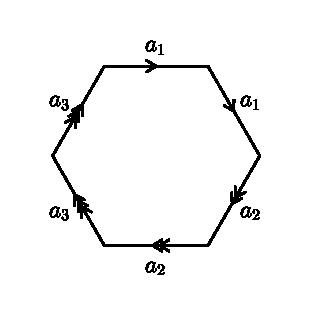
\includegraphics[width=0.5\textwidth,height=2.3in,keepaspectratio]{figs/nk.pdf}\end{center}
\begin{center}\renewcommand{\arraystretch}{1.25}\begin{tabular}{>{\raggedleft\arraybackslash}p{.17\textwidth}p{.68\textwidth}}\toprule
$\pi_1$ & $\langle a_1,\dots,a_k\mid a_1^2a_2^2\cdots a_k^2\rangle$\\ $H_*$ & $\mathbb{Z},\ \mathbb{Z}^{k-1}\oplus\mathbb{Z}/2,\ 0$\\ $\chi$ & $2-k$\\ \midrule
properties & \small compact: yes; connected: yes; path-connected: yes; Hausdorff: yes; manifold: yes; orientable: no; simply connected: no; contractible: no\\ \bottomrule\end{tabular}\end{center}
\pt{Method} A $2k$-gon with word $a_1a_1a_2a_2\cdots a_ka_k$.
\pt{Sources} Not listed in the $\pi$-Base or in Steen and Seebach.
\subsection*{Point-set properties}
\pt{Compact manifold}Polygon argument as for $\Sigma_g$.
\pt{Non-orientable}Each $a_i$ appears twice with the same exponent, so each contributes a Möbius band.
\subsection*{Algebraic invariants}
\pt{Fundamental group}One vertex, $k$ edges, one 2-cell; van Kampen gives the presentation.
\pt{Homology}$\partial e=2(a_1+\cdots+a_k)$. Change basis to $a_1,\dots,a_{k-1},s=a_1+\cdots+a_k$; then $H_1=\mathbb{Z}^{k-1}\oplus\mathbb{Z}/2$ and $H_2=0$.
\pt{Classification}$\chi=2-k$. The torsion in $H_1$ separates $N_k$ from every $\Sigma_g$, and $\chi$ separates the $N_k$ from each other.
\subsection*{Why it is in the zoo}With $\Sigma_g$ this completes the classification of closed surfaces. Exercise: $T^2\#\mathbb{RP}^2\cong N_3$.
\bigskip
\chapter{Graphs and wedges}
\entry{Figure eight}{fig8}
\noindent$S^1\vee S^1$.\enspace Two circles joined at a point.
\begin{center}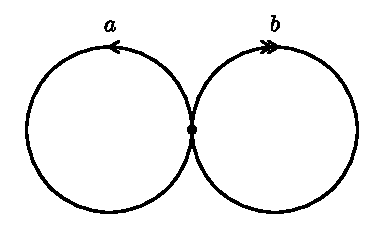
\includegraphics[width=0.5\textwidth,height=2.3in,keepaspectratio]{figs/fig8.pdf}\end{center}
\begin{center}\renewcommand{\arraystretch}{1.25}\begin{tabular}{>{\raggedleft\arraybackslash}p{.17\textwidth}p{.68\textwidth}}\toprule
$\pi_1$ & $F_2=\langle a,b\rangle$\\ $H_*$ & $\mathbb{Z},\ \mathbb{Z}^2,\ 0$\\ $\chi$ & $-1$\\ \midrule
properties & \small compact: yes; connected: yes; path-connected: yes; Hausdorff: yes; manifold: no; orientable: ---; simply connected: no; contractible: no\\ \bottomrule\end{tabular}\end{center}
\pt{Method} Van Kampen with two thickened circles meeting in a contractible cross.
\pt{Sources} Not listed in the $\pi$-Base or in Steen and Seebach.
\subsection*{Point-set properties}
\pt{Compact, Hausdorff}A union of two circles in $\mathbb{R}^2$, closed and bounded.
\pt{Not a manifold}Removing the wedge point from a small connected neighborhood of it leaves four components. In a 1-manifold the answer would be two, and in higher-dimensional manifolds one.
\subsection*{Algebraic invariants}
\pt{Van Kampen}Let $U$ be circle $A$ together with a small open arc of $B$ at the wedge point, and $V$ the reverse. $U\simeq A$, $V\simeq B$, and $U\cap V$ is a contractible cross. So $\pi_1=\mathbb{Z}*\mathbb{Z}=F_2$.
\pt{Homology}One vertex and two loops, all differentials zero: $H_1=\mathbb{Z}^2$, $\chi=1-2=-1$. The abelianization map $F_2\to\mathbb{Z}^2$ forgets the order of letters.
\pt{Universal cover}The 4-valent tree, the Cayley graph of $F_2$. It is contractible, so the figure eight is a $K(F_2,1)$.
\subsection*{Why it is in the zoo}$F_2$ is non-abelian and contains free subgroups of every countable rank. Its covering spaces are graphs one can draw.
\bigskip
\entry{Wedge of n circles}{rose}
\noindent$\bigvee_{i=1}^n S^1\ \simeq\ \mathbb{R}^2\setminus\{p_1,\dots,p_n\}$.\enspace A rose with $n$ petals. The plane minus $n$ points deformation retracts onto one.
\begin{center}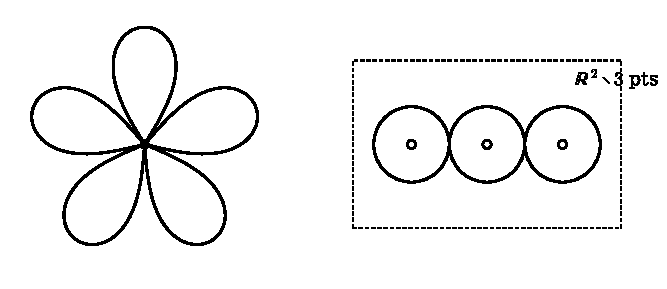
\includegraphics[width=0.82\textwidth,height=2.3in,keepaspectratio]{figs/rose.pdf}\end{center}
\begin{center}\renewcommand{\arraystretch}{1.25}\begin{tabular}{>{\raggedleft\arraybackslash}p{.17\textwidth}p{.68\textwidth}}\toprule
$\pi_1$ & $F_n$\\ $H_*$ & $\mathbb{Z},\ \mathbb{Z}^n,\ 0$\\ $\chi$ & $1-n$\\ \midrule
properties & \small compact: yes; connected: yes; path-connected: yes; Hausdorff: yes; manifold: no; orientable: ---; simply connected: no; contractible: no\\ \bottomrule\end{tabular}\end{center}
\pt{Method} Van Kampen by induction on $n$.
\pt{Sources} Not listed in the $\pi$-Base or in Steen and Seebach.
\subsection*{Point-set properties}
\pt{Wedge}Compact and Hausdorff as a finite union of circles in the plane; not a manifold at the wedge point when $n\ge2$.
\pt{Punctured plane}An open subset of $\mathbb{R}^2$, hence a non-compact orientable 2-manifold. It is a different space with the same homotopy type.
\subsection*{Algebraic invariants}
\pt{Fundamental group}Induction with van Kampen: $\pi_1(\bigvee^{n}S^1)=\pi_1(\bigvee^{n-1}S^1)*\mathbb{Z}$.
\pt{Deformation retraction}Place the punctures on a line. The plane minus the points retracts onto a chain of $n$ circles around them, which is a graph with $\chi=1-n$ and so homotopy equivalent to the rose.
\pt{Homology}$H_1=\mathbb{Z}^n$, $\chi=1-n$.
\subsection*{Why it is in the zoo}$H_1$ sees only $\mathbb{Z}^n$ and loses the non-commutativity of $F_n$.
\pt{Where it appears} The Aharonov–Bohm effect (\S\ref{app:app-ab}); Kirchhoff's laws and the cycle space of a circuit (\S\ref{app:app-kirchhoff}).
\bigskip
\entry{Finite connected graph}{graph}
\noindent$\Gamma,\ V\text{ vertices},\ E\text{ edges}$.\enspace A 1-dimensional CW complex, such as the theta graph or $K_4$.
\begin{center}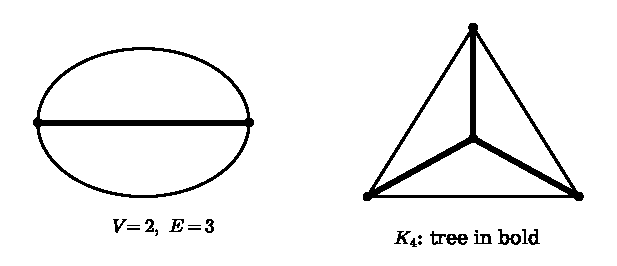
\includegraphics[width=0.82\textwidth,height=2.3in,keepaspectratio]{figs/graph.pdf}\end{center}
\begin{center}\renewcommand{\arraystretch}{1.25}\begin{tabular}{>{\raggedleft\arraybackslash}p{.17\textwidth}p{.68\textwidth}}\toprule
$\pi_1$ & $F_{E-V+1}$\\ $H_*$ & $\mathbb{Z},\ \mathbb{Z}^{E-V+1},\ 0$\\ $\chi$ & $V-E$\\ \midrule
properties & \small compact: yes; connected: yes; path-connected: yes; Hausdorff: yes; manifold: no; orientable: ---; simply connected: if a tree; contractible: no\\ \bottomrule\end{tabular}\end{center}
\pt{Method} Collapse a spanning tree; what remains is a wedge of circles.
\pt{Sources} Not listed in the $\pi$-Base or in Steen and Seebach.
\subsection*{Point-set properties}
\pt{Compact, Hausdorff}Finite CW complex.
\pt{Manifold?}Only if every vertex has degree 2, in which case $\Gamma$ is a circle.
\subsection*{Algebraic invariants}
\pt{Spanning tree}A finite connected graph contains a tree $T$ through all $V$ vertices, with $V-1$ edges. A finite tree is contractible: remove a leaf and its edge, and induct.
\pt{Collapse}For a CW pair with contractible subcomplex, $\Gamma\to\Gamma/T$ is a homotopy equivalence. $\Gamma/T$ has one vertex and $E-V+1$ loops, so $\pi_1=F_{E-V+1}$.
\pt{Homology}$\chi=V-E$ from the cell count, and $H_0=\mathbb{Z}$, so $\operatorname{rank}H_1=1-\chi=E-V+1$.
\subsection*{Why it is in the zoo}Nielsen–Schreier: every subgroup of a free group is free, because covers of graphs are graphs. Theta graph: $V=2$, $E=3$, so $F_2$.
\pt{Where it appears} Anyons and braid statistics (\S\ref{app:app-anyons}); Persistent homology and barcodes (\S\ref{app:app-barcodes}); Coverage in sensor networks (\S\ref{app:app-coverage}); Robot arms and motion planning (\S\ref{app:app-robots}); Kirchhoff's laws and the cycle space of a circuit (\S\ref{app:app-kirchhoff}).
\bigskip
\entry{Infinite wedge of circles}{infwedge}
\noindent$\bigvee_{i\in\mathbb{N}} S^1\ (\text{CW topology})$.\enspace Countably many circles at one point, with the weak topology of a CW complex.
\begin{center}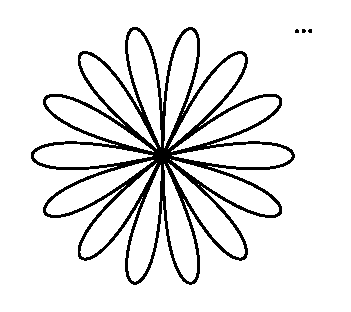
\includegraphics[width=0.5\textwidth,height=2.3in,keepaspectratio]{figs/infwedge.pdf}\end{center}
\begin{center}\renewcommand{\arraystretch}{1.25}\begin{tabular}{>{\raggedleft\arraybackslash}p{.17\textwidth}p{.68\textwidth}}\toprule
$\pi_1$ & $F_\infty$\\ $H_*$ & $\mathbb{Z},\ \bigoplus_{\mathbb{N}}\mathbb{Z},\ 0$\\ $\chi$ & $\text{undefined}$\\ \midrule
properties & \small compact: no; connected: yes; path-connected: yes; Hausdorff: yes; manifold: no; orientable: ---; simply connected: no; contractible: no\\ \bottomrule\end{tabular}\end{center}
\pt{Method} Compact images meet finitely many circles, so the group is a direct limit of the $F_n$.
\pt{Sources} $\pi$-Base \href{https://topology.pi-base.org/spaces/S000139}{S000139}.
\subsection*{Point-set properties}
\pt{Not compact}Let $U_0$ be the union of small open arcs at the wedge point on every circle, and $U_i$ the $i$-th circle minus the wedge point. The point opposite the wedge on circle $i$ lies only in $U_i$, so no finite subcover exists.
\pt{Not first countable}Given countably many neighborhoods of the wedge point, shrink the $n$-th one on circle $n$ to get a neighborhood containing none of them. So the space is not metrizable and does not embed in $\mathbb{R}^2$.
\subsection*{Algebraic invariants}
\pt{Direct limit}A compact subset of a CW complex meets only finitely many cells. Every loop and every homotopy therefore lives in a finite sub-wedge, so $\pi_1=\varinjlim F_n=F_\infty$, free on countably many generators.
\pt{Homology}Same argument: $H_1=\bigoplus_{\mathbb{N}}\mathbb{Z}$.
\subsection*{Why it is in the zoo}Compare the Hawaiian earring: the same picture with a different topology gives a different group.
\bigskip
\entry{Circle wedge sphere}{s1vs2}
\noindent$S^1\vee S^2$.\enspace A circle and a 2-sphere joined at a point.
\begin{center}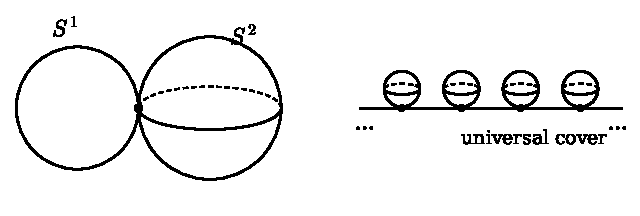
\includegraphics[width=0.82\textwidth,height=2.3in,keepaspectratio]{figs/s1vs2.pdf}\end{center}
\begin{center}\renewcommand{\arraystretch}{1.25}\begin{tabular}{>{\raggedleft\arraybackslash}p{.17\textwidth}p{.68\textwidth}}\toprule
$\pi_1$ & $\mathbb{Z}$\\ $H_*$ & $\mathbb{Z},\ \mathbb{Z},\ \mathbb{Z}$\\ $\chi$ & $1$\\ \midrule
properties & \small compact: yes; connected: yes; path-connected: yes; Hausdorff: yes; manifold: no; orientable: ---; simply connected: no; contractible: no\\ \bottomrule\end{tabular}\end{center}
\pt{Method} Van Kampen; the sphere contributes nothing.
\pt{Sources} Not listed in the $\pi$-Base or in Steen and Seebach.
\subsection*{Point-set properties}
\pt{Compact, Hausdorff}Finite CW complex.
\pt{Not a manifold}Points on the circle have 1-dimensional neighborhoods and points on the sphere 2-dimensional ones.
\subsection*{Algebraic invariants}
\pt{Fundamental group}Van Kampen: $\mathbb{Z}*1=\mathbb{Z}$.
\pt{Homology}Cells $e^0,e^1,e^2$ with zero differentials: $H=\mathbb{Z},\mathbb{Z},\mathbb{Z}$, $\chi=1$.
\pt{Second homotopy group}The universal cover is $\mathbb{R}$ with a 2-sphere attached at each integer, which is homotopy equivalent to $\bigvee_{n\in\mathbb{Z}}S^2$. Covers induce isomorphisms on $\pi_2$, and Hurewicz for the simply connected cover gives $\pi_2\cong H_2=\bigoplus_{\mathbb{Z}}\mathbb{Z}$. The deck generator $t$ shifts the spheres, so as a $\mathbb{Z}[\pi_1]$-module this is $\mathbb{Z}[t,t^{-1}]$.
\subsection*{Why it is in the zoo}$\pi_2\cong\mathbb{Z}[t,t^{-1}]$ is not finitely generated, although the space is a finite complex.
\bigskip
\entry{Moore space}{moore}
\noindent$M(\mathbb{Z}/n,1)=S^1\cup_n e^2$.\enspace A disk attached to a circle by a map of degree $n$. For $n=2$ this is $\mathbb{RP}^2$.
\begin{center}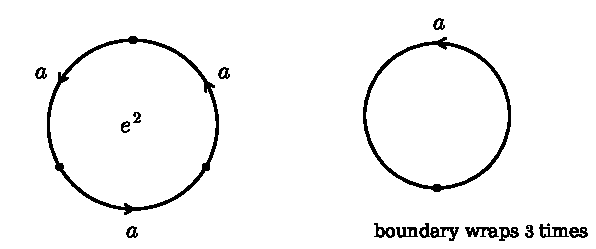
\includegraphics[width=0.82\textwidth,height=2.3in,keepaspectratio]{figs/moore.pdf}\end{center}
\begin{center}\renewcommand{\arraystretch}{1.25}\begin{tabular}{>{\raggedleft\arraybackslash}p{.17\textwidth}p{.68\textwidth}}\toprule
$\pi_1$ & $\mathbb{Z}/n$\\ $H_*$ & $\mathbb{Z},\ \mathbb{Z}/n,\ 0$\\ $\chi$ & $1$\\ \midrule
properties & \small compact: yes; connected: yes; path-connected: yes; Hausdorff: yes; manifold: no; orientable: ---; simply connected: no; contractible: no\\ \bottomrule\end{tabular}\end{center}
\pt{Method} Attaching a 2-cell along $a^n$ adds the relation $a^n=1$.
\pt{Sources} Not listed in the $\pi$-Base or in Steen and Seebach.
\subsection*{Point-set properties}
\pt{Compact, Hausdorff}Finite CW complex.
\pt{Not a manifold for $n\ge3$}Near a point of the circle, $n$ sheets of the disk meet along a line, like the pages of a book. For $n=2$ two sheets meet and the result is the manifold $\mathbb{RP}^2$.
\subsection*{Algebraic invariants}
\pt{Fundamental group}Van Kampen with the open 2-cell and the complement of its center: $\langle a\mid a^n\rangle=\mathbb{Z}/n$.
\pt{Homology}$0\to\mathbb{Z}\xrightarrow{\ n\ }\mathbb{Z}\xrightarrow{\ 0\ }\mathbb{Z}\to0$, so $H_1=\mathbb{Z}/n$ and $H_2=0$.
\subsection*{Why it is in the zoo}Attaching 2-cells kills elements of $\pi_1$. Every finitely presented group arises from a 2-complex this way.
\bigskip
\chapter{Projective spaces and Lie groups}
\entry{Real projective space}{rpn}
\noindent$\mathbb{RP}^n,\ n\ge 2$.\enspace Lines through the origin in $\mathbb{R}^{n+1}$; $S^n/\pm1$.
\begin{center}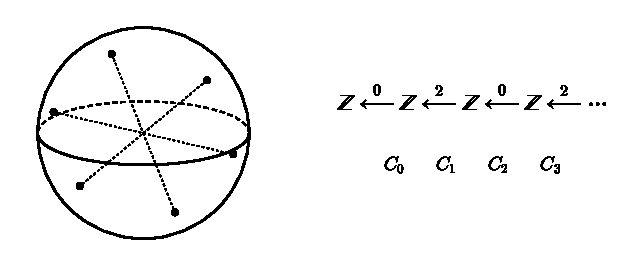
\includegraphics[width=0.82\textwidth,height=2.3in,keepaspectratio]{figs/rpn.pdf}\end{center}
\begin{center}\renewcommand{\arraystretch}{1.25}\begin{tabular}{>{\raggedleft\arraybackslash}p{.17\textwidth}p{.68\textwidth}}\toprule
$\pi_1$ & $\mathbb{Z}/2$\\ $H_*$ & $H_k=\begin{cases}\mathbb{Z} & k=0\\ \mathbb{Z}/2 & k\text{ odd},\ 0<k<n\\ 0 & k\text{ even},\ 0<k<n\\ \mathbb{Z} & k=n\text{ odd}\\ 0 & k=n\text{ even}\end{cases}$\\ $\chi$ & $\tfrac{1+(-1)^n}{2}$\\ \midrule
properties & \small compact: yes; connected: yes; path-connected: yes; Hausdorff: yes; manifold: yes; orientable: if n odd; simply connected: no; contractible: no\\ \bottomrule\end{tabular}\end{center}
\pt{Method} Universal cover $S^n$ with deck group $\{\pm1\}$; cellular differentials alternate $0$ and $2$.
\pt{Sources} Not listed in the $\pi$-Base or in Steen and Seebach.
\subsection*{Point-set properties}
\pt{Compact, Hausdorff, manifold}Same argument as for $\mathbb{RP}^2$: a quotient of $S^n$ by a free action of a finite group.
\pt{Orientability}The antipodal map of $S^n$ has degree $(-1)^{n+1}$. It preserves orientation, so the orientation descends to the quotient, exactly when $n$ is odd.
\subsection*{Algebraic invariants}
\pt{Fundamental group}For $n\ge2$, $S^n$ is simply connected, so $\pi_1\cong\{\pm1\}$.
\pt{Cell structure}$\mathbb{RP}^n=\mathbb{RP}^{n-1}\cup e^n$, with $e^n$ attached by the double cover $S^{n-1}\to\mathbb{RP}^{n-1}$. One cell in each dimension $0,\dots,n$.
\pt{Differentials}The cellular differential $d_k$ is the degree of the attaching map followed by collapsing $\mathbb{RP}^{k-2}$. This is $1+(-1)^k$: zero for $k$ odd, two for $k$ even. The chain complex is $\mathbb{Z}\xleftarrow{0}\mathbb{Z}\xleftarrow{2}\mathbb{Z}\xleftarrow{0}\mathbb{Z}\xleftarrow{2}\cdots$, which gives the table.
\pt{Euler characteristic}$\chi=\sum_{k=0}^n(-1)^k$, which is $1$ for $n$ even and $0$ for $n$ odd, consistent with $\chi(S^n)=2\chi(\mathbb{RP}^n)$.
\subsection*{Why it is in the zoo}The standard cellular homology exercise. Orientable exactly when $n$ is odd.
\pt{Where it appears} Borsuk–Ulam: antipodes and fair division (\S\ref{app:app-borsuk}).
\bigskip
\entry{Rotation group}{so3}
\noindent$SO(3)\cong\mathbb{RP}^3$.\enspace Rotations of $\mathbb{R}^3$; a ball of radius $\pi$ with antipodal boundary points identified.
\begin{center}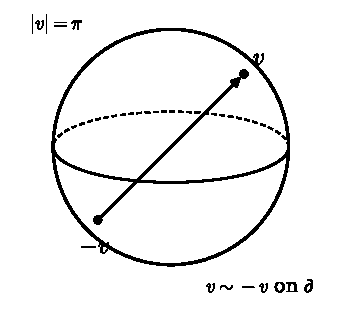
\includegraphics[width=0.5\textwidth,height=2.3in,keepaspectratio]{figs/so3.pdf}\end{center}
\begin{center}\renewcommand{\arraystretch}{1.25}\begin{tabular}{>{\raggedleft\arraybackslash}p{.17\textwidth}p{.68\textwidth}}\toprule
$\pi_1$ & $\mathbb{Z}/2$\\ $H_*$ & $\mathbb{Z},\ \mathbb{Z}/2,\ 0,\ \mathbb{Z}$\\ $\chi$ & $0$\\ \midrule
properties & \small compact: yes; connected: yes; path-connected: yes; Hausdorff: yes; manifold: yes; orientable: yes; simply connected: no; contractible: no\\ \bottomrule\end{tabular}\end{center}
\pt{Method} Double cover $SU(2)\cong S^3\to SO(3)$ by unit quaternions.
\pt{Sources} Not listed in the $\pi$-Base or in Steen and Seebach.
\subsection*{Point-set properties}
\pt{Compact}$SO(3)$ is closed ($A^TA=I$, $\det A=1$) and bounded (entries in $[-1,1]$) in $\mathbb{R}^9$.
\pt{Manifold, orientable}$I$ is a regular value of $A\mapsto A^TA$ on $GL_3^+$, so $SO(3)$ is a 3-manifold. Lie groups are parallelizable (translate a frame at $I$), hence orientable.
\pt{The ball model}Send $v$ in the ball of radius $\pi$ to the rotation about $v$ by angle $|v|$. This is a bijection except that $v$ and $-v$ with $|v|=\pi$ give the same rotation, so $SO(3)\cong D^3/(v\sim-v\text{ on }\partial D^3)\cong\mathbb{RP}^3$.
\subsection*{Algebraic invariants}
\pt{Covering}Unit quaternions $q$ act on pure quaternions $\mathbb{R}^3$ by $v\mapsto qvq^{-1}$, a rotation. The kernel of $S^3\to SO(3)$ is $\{\pm1\}$. Since $S^3$ is simply connected, $\pi_1(SO(3))\cong\mathbb{Z}/2$.
\pt{The nontrivial loop}In the ball model, a diameter from $v$ to $-v$ is a loop. Its lift to $S^3$ runs from $q$ to $-q$ and does not close. Running it twice does close up, and is null-homotopic.
\pt{Homology}From $\mathbb{RP}^3$: $\mathbb{Z},\mathbb{Z}/2,0,\mathbb{Z}$, and $\chi=0$.
\subsection*{Why it is in the zoo}The plate trick: a rotation by $2\pi$ is not null-homotopic but a rotation by $4\pi$ is. $SO(n)$ has $\pi_1=\mathbb{Z}/2$ for every $n\ge3$.
\pt{Where it appears} Spin one-half and the belt trick (\S\ref{app:app-spin}); Instantons and the vacuum of gauge theory (\S\ref{app:app-instanton}); Orientations, gimbal lock, and quaternions (\S\ref{app:app-attitude}).
\bigskip
\entry{Unitary group}{un}
\noindent$U(n)$.\enspace Complex $n\times n$ matrices with $A^*A=I$. $U(1)=S^1$.
\begin{center}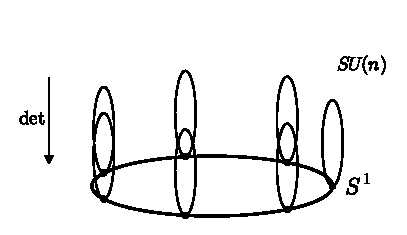
\includegraphics[width=0.5\textwidth,height=2.3in,keepaspectratio]{figs/un.pdf}\end{center}
\begin{center}\renewcommand{\arraystretch}{1.25}\begin{tabular}{>{\raggedleft\arraybackslash}p{.17\textwidth}p{.68\textwidth}}\toprule
$\pi_1$ & $\mathbb{Z}$\\ $H_*$ & $H_*\cong\Lambda_{\mathbb{Z}}[x_1,x_3,\dots,x_{2n-1}]$\\ $\chi$ & $0$\\ \midrule
properties & \small compact: yes; connected: yes; path-connected: yes; Hausdorff: yes; manifold: yes; orientable: yes; simply connected: no; contractible: no\\ \bottomrule\end{tabular}\end{center}
\pt{Method} $\det:U(n)\to S^1$ with simply connected fiber $SU(n)$.
\pt{Sources} Not listed in the $\pi$-Base or in Steen and Seebach.
\subsection*{Point-set properties}
\pt{Compact, manifold}Closed and bounded in $\mathbb{C}^{n^2}$; a Lie group of real dimension $n^2$.
\pt{Connected}Every unitary matrix is $V\operatorname{diag}(e^{i\theta_1},\dots,e^{i\theta_n})V^*$. Shrinking all $\theta_j$ to $0$ gives a path to $I$.
\subsection*{Algebraic invariants}
\pt{Splitting}As spaces, $U(n)\cong SU(n)\times S^1$ via $A\mapsto(A\operatorname{diag}(\det A^{-1},1,\dots,1),\det A)$.
\pt{$SU(n)$ is simply connected}$SU(n)$ acts transitively on the unit sphere $S^{2n-1}\subset\mathbb{C}^n$ with stabilizer $SU(n-1)$. The fibration $SU(n-1)\to SU(n)\to S^{2n-1}$ and $\pi_1(S^{2n-1})=\pi_2(S^{2n-1})=0$ give $\pi_1SU(n)\cong\pi_1SU(n-1)$, down to $SU(1)=1$.
\pt{Conclusion}$\pi_1(U(n))\cong\pi_1(S^1)=\mathbb{Z}$, detected by the determinant.
\pt{Homology}The cohomology ring is an exterior algebra on classes of degrees $1,3,\dots,2n-1$, so total rank is $2^n$ and $\chi=\prod(1-1)=0$.
\subsection*{Why it is in the zoo}The long exact sequence of a fibration is the natural tool here. Total rank of homology is $2^n$.
\pt{Where it appears} The Dirac monopole and charge quantization (\S\ref{app:app-monopole}); Instantons and the vacuum of gauge theory (\S\ref{app:app-instanton}).
\bigskip
\entry{General linear group}{gln}
\noindent$GL_n(\mathbb{R})$.\enspace Invertible real $n\times n$ matrices, an open subset of $\mathbb{R}^{n^2}$.
\begin{center}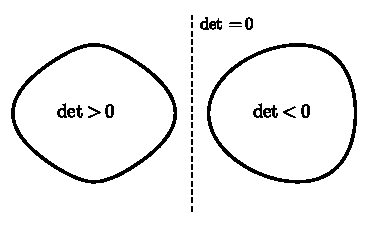
\includegraphics[width=0.5\textwidth,height=2.3in,keepaspectratio]{figs/gln.pdf}\end{center}
\begin{center}\renewcommand{\arraystretch}{1.25}\begin{tabular}{>{\raggedleft\arraybackslash}p{.17\textwidth}p{.68\textwidth}}\toprule
$\pi_1$ & $\pi_1(GL_n^+)=\mathbb{Z}\ (n=2),\ \ \mathbb{Z}/2\ (n\ge3)$\\ $H_*$ & $\text{two copies of }H_*(SO(n))$\\ $\chi$ & $0$\\ \midrule
properties & \small compact: no; connected: no; path-connected: no; Hausdorff: yes; manifold: yes; orientable: yes; simply connected: ---; contractible: no\\ \bottomrule\end{tabular}\end{center}
\pt{Method} Gram–Schmidt retracts $GL_n(\mathbb{R})$ onto $O(n)$.
\pt{Sources} Not listed in the $\pi$-Base or in Steen and Seebach.
\subsection*{Point-set properties}
\pt{Open manifold}$\det$ is continuous, so $\{\det\ne0\}$ is open in $\mathbb{R}^{n^2}$.
\pt{Not compact}$tI$ for $t\to\infty$ is unbounded.
\pt{Two components}$\det$ maps onto $\mathbb{R}\setminus\{0\}$, which is disconnected, so $GL_n$ is too. Each half is connected because it retracts onto $SO(n)$ or its translate.
\subsection*{Algebraic invariants}
\pt{Gram–Schmidt}Every $A$ factors uniquely as $A=QR$ with $Q\in O(n)$ and $R$ upper triangular with positive diagonal. The space of such $R$ is convex, so $GL_n\simeq O(n)=SO(n)\sqcup(\text{reflection})\cdot SO(n)$.
\pt{Fundamental group}$SO(2)=S^1$ gives $\mathbb{Z}$. For $n\ge3$, the fibration $SO(n-1)\to SO(n)\to S^{n-1}$ gives $\pi_1SO(n)\cong\pi_1SO(3)=\mathbb{Z}/2$.
\subsection*{Why it is in the zoo}Disconnected by the sign of the determinant, which is why orientation is a binary choice.
\bigskip
\entry{Complex projective space}{cpn}
\noindent$\mathbb{CP}^n$.\enspace Complex lines in $\mathbb{C}^{n+1}$; $S^{2n+1}/S^1$. $\mathbb{CP}^1=S^2$.
\begin{center}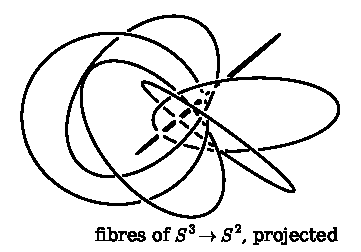
\includegraphics[width=0.5\textwidth,height=2.3in,keepaspectratio]{figs/cpn.pdf}\end{center}
\begin{center}\renewcommand{\arraystretch}{1.25}\begin{tabular}{>{\raggedleft\arraybackslash}p{.17\textwidth}p{.68\textwidth}}\toprule
$\pi_1$ & $1$\\ $H_*$ & $H_{2k}=\mathbb{Z}\ (0\le k\le n),\ \text{odd degrees }0$\\ $\chi$ & $n+1$\\ \midrule
properties & \small compact: yes; connected: yes; path-connected: yes; Hausdorff: yes; manifold: yes; orientable: yes; simply connected: yes; contractible: no\\ \bottomrule\end{tabular}\end{center}
\pt{Method} One cell in each even dimension, so no 1-cells.
\pt{Sources} Not listed in the $\pi$-Base or in Steen and Seebach.
\subsection*{Point-set properties}
\pt{Compact, Hausdorff}Quotient of $S^{2n+1}$ by the free action of the compact group $S^1$.
\pt{Manifold, orientable}Affine charts $\{z_i\ne0\}\cong\mathbb{C}^n$ with holomorphic transitions. Complex manifolds are orientable because complex-linear maps have positive real determinant $|\det|^2$.
\subsection*{Algebraic invariants}
\pt{Cell structure}The points with $z_n\ne0$ can be normalized to $z_n$ real and positive, leaving $(z_0,\dots,z_{n-1})$ in an open $2n$-ball. So $\mathbb{CP}^n=\mathbb{CP}^{n-1}\cup e^{2n}$.
\pt{Homology and $\pi_1$}Cells only in even degrees, so all differentials are zero and $H_{2k}=\mathbb{Z}$. The 2-skeleton is $S^2$, and $\pi_1$ depends only on the 2-skeleton, so $\pi_1=1$. $\chi=n+1$.
\pt{Hopf fibration}The long exact sequence of $S^1\to S^3\to S^2$ gives $\pi_3(S^2)\cong\pi_3(S^3)=\mathbb{Z}$. Any two fibers are linked circles.
\subsection*{Why it is in the zoo}All cellular differentials vanish for parity reasons. The Hopf fibration $S^1\to S^3\to\mathbb{CP}^1$ gives $\pi_3(S^2)\cong\mathbb{Z}$.
\pt{Where it appears} The Dirac monopole and charge quantization (\S\ref{app:app-monopole}); The quantum Hall effect and Chern numbers (\S\ref{app:app-hall}); Qubits, the Bloch sphere, and geometric phase (\S\ref{app:app-bloch}).
\bigskip
\entry{Quaternionic projective space}{hpn}
\noindent$\mathbb{HP}^n$.\enspace Quaternionic lines in $\mathbb{H}^{n+1}$. $\mathbb{HP}^1=S^4$.
\begin{center}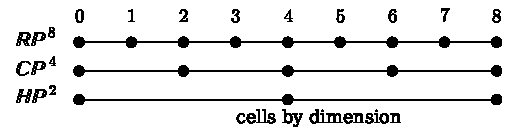
\includegraphics[width=0.82\textwidth,height=2.3in,keepaspectratio]{figs/hpn.pdf}\end{center}
\begin{center}\renewcommand{\arraystretch}{1.25}\begin{tabular}{>{\raggedleft\arraybackslash}p{.17\textwidth}p{.68\textwidth}}\toprule
$\pi_1$ & $1$\\ $H_*$ & $H_{4k}=\mathbb{Z}\ (0\le k\le n),\ \text{else }0$\\ $\chi$ & $n+1$\\ \midrule
properties & \small compact: yes; connected: yes; path-connected: yes; Hausdorff: yes; manifold: yes; orientable: yes; simply connected: yes; contractible: no\\ \bottomrule\end{tabular}\end{center}
\pt{Method} One cell in each dimension divisible by 4.
\pt{Sources} Not listed in the $\pi$-Base or in Steen and Seebach.
\subsection*{Point-set properties}
\pt{Compact manifold}Quotient of $S^{4n+3}$ by the free action of the unit quaternions $S^3$; real dimension $4n$, orientable.
\subsection*{Algebraic invariants}
\pt{Cells}Same normalization as for $\mathbb{CP}^n$ with quaternions: $\mathbb{HP}^n=\mathbb{HP}^{n-1}\cup e^{4n}$. Differentials vanish, and the 3-skeleton is a point, so $\pi_1=\pi_2=\pi_3=1$. $\chi=n+1$.
\subsection*{Why it is in the zoo}Source of the Hopf fibration $S^3\to S^7\to S^4$, so $\pi_7(S^4)$ contains $\mathbb{Z}$.
\bigskip
\chapter{Three-manifolds}
\entry{Lens space}{lens}
\noindent$L(p,q)$.\enspace $S^3/(\mathbb{Z}/p)$ with the generator acting by $(z,w)\mapsto(e^{2\pi i/p}z,\,e^{2\pi iq/p}w)$, $\gcd(p,q)=1$. Also two solid tori glued along their boundary.
\begin{center}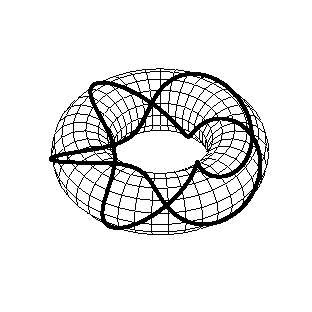
\includegraphics[width=0.5\textwidth,height=2.3in,keepaspectratio]{figs/lens.pdf}\end{center}
\begin{center}\renewcommand{\arraystretch}{1.25}\begin{tabular}{>{\raggedleft\arraybackslash}p{.17\textwidth}p{.68\textwidth}}\toprule
$\pi_1$ & $\mathbb{Z}/p$\\ $H_*$ & $\mathbb{Z},\ \mathbb{Z}/p,\ 0,\ \mathbb{Z}$\\ $\chi$ & $0$\\ \midrule
properties & \small compact: yes; connected: yes; path-connected: yes; Hausdorff: yes; manifold: yes; orientable: yes; simply connected: no; contractible: no\\ \bottomrule\end{tabular}\end{center}
\pt{Method} A free action on the simply connected $S^3$.
\pt{Sources} Not listed in the $\pi$-Base or in Steen and Seebach.
\subsection*{Point-set properties}
\pt{Compact orientable 3-manifold}The action is free because $\gcd(p,q)=1$, so no nonidentity element fixes a point of $S^3$. It is by unitary matrices, which preserve orientation, so the quotient is an orientable manifold.
\pt{Heegaard picture}Split $S^3$ into $|z|\le|w|$ and $|z|\ge|w|$, two solid tori. The action preserves both, and $L(p,q)$ is two solid tori glued so that a meridian of one goes to a curve winding $p$ times one way and $q$ times the other on the boundary torus of the second.
\subsection*{Algebraic invariants}
\pt{Fundamental group}$S^3\to L(p,q)$ is a $p$-sheeted universal covering, so $\pi_1\cong\mathbb{Z}/p$.
\pt{Homology}There is a CW structure with one cell in each dimension $0$ to $3$ and differentials $0,\ p,\ 0$. So $H=\mathbb{Z},\mathbb{Z}/p,0,\mathbb{Z}$, and $\chi=0$ as for every closed odd-dimensional manifold.
\pt{Classification}$L(p,q)\simeq L(p,q')$ iff $qq'\equiv\pm n^2\pmod p$ for some $n$; homeomorphic iff $q'\equiv\pm q^{\pm1}\pmod p$. The squares mod 5 are $1,4$, so $L(5,1)\not\simeq L(5,2)$. Mod 7, $2\equiv3^2$, so $L(7,1)\simeq L(7,2)$, but $2\not\equiv\pm1^{\pm1}$ and $2^{-1}=4\not\equiv\pm1$, so they are not homeomorphic.
\subsection*{Why it is in the zoo}$L(5,1)$ and $L(5,2)$ have the same $\pi_1$ and homology but are not homotopy equivalent. $L(7,1)$ and $L(7,2)$ are homotopy equivalent but not homeomorphic.
\pt{Where it appears} The shape of the universe (\S\ref{app:app-cosmic}).
\bigskip
\entry{Poincaré homology sphere}{poincare}
\noindent$\Sigma(2,3,5)=S^3/I^*$.\enspace A solid dodecahedron with opposite faces glued after a twist of $\pi/5$.
\begin{center}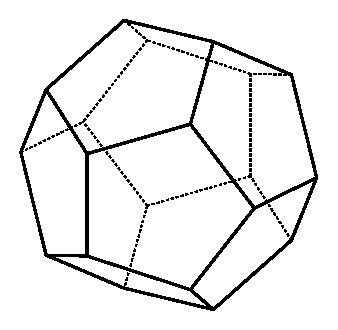
\includegraphics[width=0.5\textwidth,height=2.3in,keepaspectratio]{figs/poincare.pdf}\end{center}
\begin{center}\renewcommand{\arraystretch}{1.25}\begin{tabular}{>{\raggedleft\arraybackslash}p{.17\textwidth}p{.68\textwidth}}\toprule
$\pi_1$ & $I^*=\langle s,t\mid (st)^2=s^3=t^5\rangle,\ |I^*|=120$\\ $H_*$ & $\mathbb{Z},\ 0,\ 0,\ \mathbb{Z}$\\ $\chi$ & $0$\\ \midrule
properties & \small compact: yes; connected: yes; path-connected: yes; Hausdorff: yes; manifold: yes; orientable: yes; simply connected: no; contractible: no\\ \bottomrule\end{tabular}\end{center}
\pt{Method} $S^3$ modulo the binary icosahedral group, acting freely by unit quaternions.
\pt{Sources} Not listed in the $\pi$-Base or in Steen and Seebach.
\subsection*{Point-set properties}
\pt{Compact orientable 3-manifold}Quotient of $S^3$ by a free action of a finite group of orientation-preserving isometries.
\subsection*{Algebraic invariants}
\pt{Fundamental group}$I^*\subset S^3$ is the preimage of the rotation group $A_5$ of the icosahedron under $S^3\to SO(3)$, of order $2\cdot60=120$. The covering $S^3\to S^3/I^*$ gives $\pi_1\cong I^*$.
\pt{Perfect group}Abelianize: $2s+2t=3s=5t$. From $2s+2t=3s$ get $s=2t$; then $3s=6t=5t$ gives $t=0$ and $s=0$. So $H_1=I^*/[I^*,I^*]=0$.
\pt{Remaining homology}Closed and orientable, so $H_3=\mathbb{Z}$. Poincaré duality and universal coefficients give $H_2\cong H^1=\operatorname{Hom}(H_1,\mathbb{Z})=0$.
\subsection*{Why it is in the zoo}Same homology as $S^3$ but not simply connected. This is why the Poincaré conjecture is stated with $\pi_1$.
\pt{Where it appears} The shape of the universe (\S\ref{app:app-cosmic}).
\bigskip
\entry{Circle times sphere}{s1s2}
\noindent$S^1\times S^2$.\enspace $S^2\times[0,1]$ with the two ends glued by the identity.
\begin{center}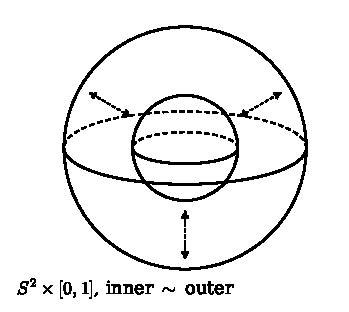
\includegraphics[width=0.5\textwidth,height=2.3in,keepaspectratio]{figs/s1s2.pdf}\end{center}
\begin{center}\renewcommand{\arraystretch}{1.25}\begin{tabular}{>{\raggedleft\arraybackslash}p{.17\textwidth}p{.68\textwidth}}\toprule
$\pi_1$ & $\mathbb{Z}$\\ $H_*$ & $\mathbb{Z},\ \mathbb{Z},\ \mathbb{Z},\ \mathbb{Z}$\\ $\chi$ & $0$\\ \midrule
properties & \small compact: yes; connected: yes; path-connected: yes; Hausdorff: yes; manifold: yes; orientable: yes; simply connected: no; contractible: no\\ \bottomrule\end{tabular}\end{center}
\pt{Method} Product formula.
\pt{Sources} Not listed in the $\pi$-Base or in Steen and Seebach.
\subsection*{Point-set properties}
\pt{Compact orientable 3-manifold}Product of compact orientable manifolds.
\subsection*{Algebraic invariants}
\pt{Fundamental group}$\pi_1(S^1)\times\pi_1(S^2)=\mathbb{Z}$.
\pt{Künneth}$H_k=\bigoplus_{i+j=k}H_i(S^1)\otimes H_j(S^2)$ with no torsion terms: $\mathbb{Z}$ in degrees $0,1,2,3$. $\chi=0\cdot2=0$.
\subsection*{Why it is in the zoo}Compare $S^1\vee S^2$: same $\pi_1$, different homology. It is prime but not irreducible, since $\{*\}\times S^2$ does not bound a ball.
\bigskip
\chapter{Knots and configurations}
\entry{Unknot and Hopf link complements}{hopflink}
\noindent$S^3\setminus U\simeq S^1,\ \ S^3\setminus H\simeq T^2$.\enspace The complement of an unknotted circle, and of two linked circles.
\begin{center}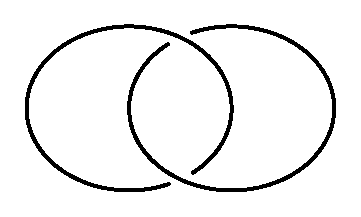
\includegraphics[width=0.5\textwidth,height=2.3in,keepaspectratio]{figs/hopflink.pdf}\end{center}
\begin{center}\renewcommand{\arraystretch}{1.25}\begin{tabular}{>{\raggedleft\arraybackslash}p{.17\textwidth}p{.68\textwidth}}\toprule
$\pi_1$ & $\mathbb{Z}\ \text{and}\ \mathbb{Z}^2$\\ $H_*$ & $(\mathbb{Z},\mathbb{Z},0)\ \text{and}\ (\mathbb{Z},\mathbb{Z}^2,\mathbb{Z})$\\ $\chi$ & $0$\\ \midrule
properties & \small compact: no; connected: yes; path-connected: yes; Hausdorff: yes; manifold: yes; orientable: yes; simply connected: no; contractible: no\\ \bottomrule\end{tabular}\end{center}
\pt{Method} $S^3$ is two solid tori; remove their cores.
\pt{Sources} Not listed in the $\pi$-Base or in Steen and Seebach.
\subsection*{Point-set properties}
\pt{Open 3-manifolds}Complements of closed subsets of $S^3$ are open, hence non-compact orientable 3-manifolds.
\subsection*{Algebraic invariants}
\pt{Unknot}$S^3=V_1\cup V_2$, two solid tori glued along a torus. Removing the core of $V_2$ leaves $V_2$ minus core $\cong T^2\times[0,1)$, which retracts onto $\partial V_1$. So $S^3\setminus U\simeq V_1\simeq S^1$.
\pt{Hopf link}The cores of $V_1$ and $V_2$ form a Hopf link. Removing both leaves $T^2\times(0,1)\simeq T^2$, so $\pi_1=\mathbb{Z}^2$, generated by the two meridians.
\pt{Unlink}A separating sphere splits the complement; van Kampen gives $\mathbb{Z}*\mathbb{Z}=F_2$, which is not $\mathbb{Z}^2$. Both have $H_1=\mathbb{Z}^2$, so homology alone does not detect linking here; $\pi_1$ does.
\subsection*{Why it is in the zoo}Two circles are linked when the complement's group is $\mathbb{Z}^2$; the unlink gives $F_2$.
\bigskip
\entry{Trefoil complement}{trefoil}
\noindent$S^3\setminus 3_1$.\enspace The complement of the simplest nontrivial knot.
\begin{center}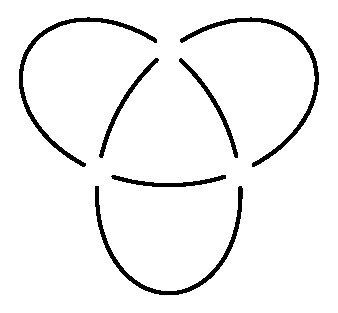
\includegraphics[width=0.5\textwidth,height=2.3in,keepaspectratio]{figs/trefoil.pdf}\end{center}
\begin{center}\renewcommand{\arraystretch}{1.25}\begin{tabular}{>{\raggedleft\arraybackslash}p{.17\textwidth}p{.68\textwidth}}\toprule
$\pi_1$ & $\langle a,b\mid aba=bab\rangle\cong\langle x,y\mid x^2=y^3\rangle$\\ $H_*$ & $\mathbb{Z},\ \mathbb{Z},\ 0$\\ $\chi$ & $0$\\ \midrule
properties & \small compact: no; connected: yes; path-connected: yes; Hausdorff: yes; manifold: yes; orientable: yes; simply connected: no; contractible: no\\ \bottomrule\end{tabular}\end{center}
\pt{Method} Wirtinger presentation from a diagram: a generator per arc, a relation per crossing.
\pt{Sources} Not listed in the $\pi$-Base or in Steen and Seebach.
\subsection*{Point-set properties}
\pt{Open 3-manifold}Open subset of $S^3$; non-compact, orientable.
\subsection*{Algebraic invariants}
\pt{Wirtinger presentation}The standard diagram has arcs $x_1,x_2,x_3$ and three crossings. Each crossing gives a relation of the form $x_{i+1}=x_i^{\pm1}x_jx_i^{\mp1}$; one relation is redundant. With suitable orientations: $x_3=x_2^{-1}x_1x_2$ and $x_1x_2x_1=x_2x_1x_2$.
\pt{Two presentations}With $a=x_1$, $b=x_2$: $\langle a,b\mid aba=bab\rangle$, the braid group $B_3$. Put $x=aba$ and $y=ab$. Then $y^3=ababab=(aba)(bab)=(aba)(aba)=x^2$.
\pt{Knotted}$a\mapsto(12)$, $b\mapsto(23)$ satisfies $aba=(13)=bab$, so the group surjects onto the non-abelian $S_3$. The unknot group $\mathbb{Z}$ has only abelian quotients.
\pt{Homology}Alexander duality: $\tilde H_k(S^3\setminus K)\cong\tilde H^{2-k}(K)=\tilde H^{2-k}(S^1)$, so $H_1=\mathbb{Z}$ and $H_2=0$ for every knot.
\subsection*{Why it is in the zoo}Every knot complement has $H_1=\mathbb{Z}$, so homology cannot detect knotting. $\pi_1$ can: this group maps onto $S_3$, which $\mathbb{Z}$ cannot.
\bigskip
\entry{Configuration space}{conf}
\noindent$\mathrm{UConf}_n(\mathbb{C})$.\enspace Unordered sets of $n$ distinct points in the plane. The ordered version is $\mathrm{Conf}_n(\mathbb{C})$.
\begin{center}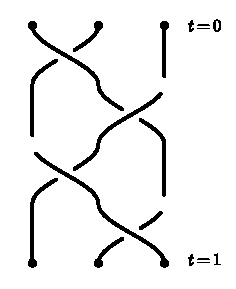
\includegraphics[width=0.5\textwidth,height=2.3in,keepaspectratio]{figs/conf.pdf}\end{center}
\begin{center}\renewcommand{\arraystretch}{1.25}\begin{tabular}{>{\raggedleft\arraybackslash}p{.17\textwidth}p{.68\textwidth}}\toprule
$\pi_1$ & $B_n\ \ (\text{ordered: } P_n)$\\ $H_*$ & $H_1=\mathbb{Z}\ (n\ge2)$\\ $\chi$ & $0\ (n\ge2)$\\ \midrule
properties & \small compact: no; connected: yes; path-connected: yes; Hausdorff: yes; manifold: yes; orientable: yes; simply connected: no; contractible: no\\ \bottomrule\end{tabular}\end{center}
\pt{Method} A loop is a motion of points that returns to the same set: a braid.
\pt{Sources} Not listed in the $\pi$-Base or in Steen and Seebach.
\subsection*{Point-set properties}
\pt{Manifold}$\mathrm{Conf}_n(\mathbb{C})$ is $\mathbb{C}^n$ minus the diagonals $z_i=z_j$, an open set. $S_n$ acts freely, so the quotient is a complex $n$-dimensional manifold, hence orientable.
\pt{Connected}The diagonals have real codimension $2$, so their complement is connected; any two configurations can be joined by moving points around each other.
\subsection*{Algebraic invariants}
\pt{Fadell–Neuwirth}Forgetting the last point, $\mathrm{Conf}_n\to\mathrm{Conf}_{n-1}$ is a fibration with fiber $\mathbb{C}$ minus $n-1$ points, a $K(F_{n-1},1)$. Induction and the long exact sequence show $\mathrm{Conf}_n$ is aspherical, with $\pi_1=P_n$ the pure braid group.
\pt{Unordered}$\mathrm{Conf}_n\to\mathrm{UConf}_n$ is an $n!$-sheeted cover, so $\pi_1=B_n$ with $1\to P_n\to B_n\to S_n\to1$.
\pt{Homology}Artin generators $\sigma_i$ satisfy $\sigma_i\sigma_{i+1}\sigma_i=\sigma_{i+1}\sigma_i\sigma_{i+1}$; abelianizing gives $\sigma_i=\sigma_{i+1}$, so $H_1=\mathbb{Z}$.
\pt{Euler characteristic}Multiplicative in fibrations: $\chi(\mathrm{Conf}_n)=\prod_{k=1}^{n-1}(1-k)=0$ for $n\ge2$, and $\chi(\mathrm{UConf}_n)=0/n!=0$.
\subsection*{Why it is in the zoo}A finite-dimensional $K(B_n,1)$. Motion of points in the plane gives braids, not permutations.
\pt{Where it appears} Anyons and braid statistics (\S\ref{app:app-anyons}); Robot arms and motion planning (\S\ref{app:app-robots}).
\bigskip
\entry{Exterior of the Alexander horned sphere}{horned}
\noindent$S^3\setminus\overline{B}$.\enspace The outer side of a wild embedding of $S^2$ in $S^3$, built from infinitely nested pairs of interlocked horns.
\begin{center}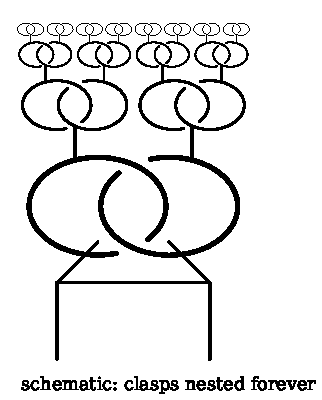
\includegraphics[width=0.5\textwidth,height=2.3in,keepaspectratio]{figs/horned.pdf}\end{center}
\begin{center}\renewcommand{\arraystretch}{1.25}\begin{tabular}{>{\raggedleft\arraybackslash}p{.17\textwidth}p{.68\textwidth}}\toprule
$\pi_1$ & $\ne 1,\ \text{perfect, infinitely generated}$\\ $H_*$ & $\mathbb{Z},\ 0,\ 0,\ 0$\\ $\chi$ & $1$\\ \midrule
properties & \small compact: no; connected: yes; path-connected: yes; Hausdorff: yes; manifold: yes; orientable: yes; simply connected: no; contractible: no\\ \bottomrule\end{tabular}\end{center}
\pt{Method} A direct limit over the stages of the construction; Alexander duality for homology.
\pt{Sources} Not listed in the $\pi$-Base or in Steen and Seebach.
\subsection*{Point-set properties}
\pt{Open 3-manifold}The complement of a compact set in $S^3$ is open; it is non-compact and orientable.
\pt{The sphere itself}The horned sphere is homeomorphic to $S^2$, and its inside is homeomorphic to an open ball. Only the outside is strange.
\subsection*{Algebraic invariants}
\pt{Homology}Alexander duality for an embedded $S^2$: $\tilde H_k(S^3\setminus S)\cong\check H^{2-k}(S^2)$ reduced, which is $\mathbb{Z}$ in degree $0$ and zero otherwise. So there are two components, each with the homology of a point.
\pt{Fundamental group}A small loop around the base of a horn cannot be slid off: at every stage it is caught by the next interlocked pair. The group is the direct limit of free groups on $2^k$ generators under maps that are injective but not surjective. It is nontrivial and not finitely generated; it is perfect since $H_1=0$.
\subsection*{Why it is in the zoo}The Schoenflies theorem fails in dimension 3. The space is acyclic yet not simply connected.
\bigskip
\chapter{Classifying spaces and complexes}
\entry{Infinite sphere}{sinf}
\noindent$S^\infty$.\enspace The union $S^0\subset S^1\subset S^2\subset\cdots$ with the weak topology.
\begin{center}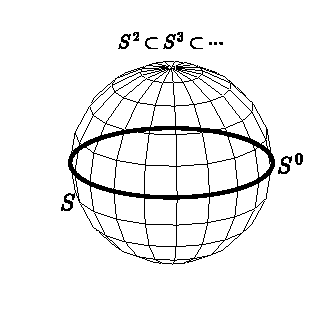
\includegraphics[width=0.5\textwidth,height=2.3in,keepaspectratio]{figs/sinf.pdf}\end{center}
\begin{center}\renewcommand{\arraystretch}{1.25}\begin{tabular}{>{\raggedleft\arraybackslash}p{.17\textwidth}p{.68\textwidth}}\toprule
$\pi_1$ & $1$\\ $H_*$ & $\mathbb{Z},\ 0,\dots$\\ $\chi$ & $1$\\ \midrule
properties & \small compact: no; connected: yes; path-connected: yes; Hausdorff: yes; manifold: no; orientable: ---; simply connected: yes; contractible: yes\\ \bottomrule\end{tabular}\end{center}
\pt{Method} Every compact image lies in some finite sphere and misses a point there.
\pt{Sources} Not listed in the $\pi$-Base or in Steen and Seebach.
\subsection*{Point-set properties}
\pt{Not compact}A compact subset of a CW complex lies in a finite subcomplex, and $S^\infty$ is not a finite subcomplex of itself.
\pt{Hausdorff}CW complexes are Hausdorff (even normal).
\subsection*{Algebraic invariants}
\pt{All homotopy groups vanish}A map $S^k\to S^\infty$ lands in some $S^n$; enlarging $n$ to exceed $k$, cellular approximation lets it miss a point of $S^n$, and $S^n$ minus a point is contractible.
\pt{Contractible}Whitehead's theorem: a CW complex with all $\pi_k=0$ is contractible.
\subsection*{Why it is in the zoo}An infinite-dimensional contractible space with free actions of $\mathbb{Z}/2$ and $S^1$. It is the total space of the next two entries.
\bigskip
\entry{Infinite real projective space}{rpinf}
\noindent$\mathbb{RP}^\infty=K(\mathbb{Z}/2,1)$.\enspace $S^\infty/\pm1$.
\begin{center}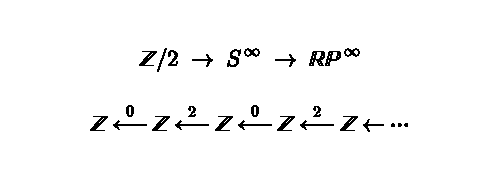
\includegraphics[width=0.5\textwidth,height=2.3in,keepaspectratio]{figs/rpinf.pdf}\end{center}
\begin{center}\renewcommand{\arraystretch}{1.25}\begin{tabular}{>{\raggedleft\arraybackslash}p{.17\textwidth}p{.68\textwidth}}\toprule
$\pi_1$ & $\mathbb{Z}/2$\\ $H_*$ & $H_k=\mathbb{Z}/2\ (k\text{ odd}),\ 0\ (k>0\text{ even})$\\ $\chi$ & $\text{undefined}$\\ \midrule
properties & \small compact: no; connected: yes; path-connected: yes; Hausdorff: yes; manifold: no; orientable: ---; simply connected: no; contractible: no\\ \bottomrule\end{tabular}\end{center}
\pt{Method} Contractible universal cover $S^\infty$ with deck group $\mathbb{Z}/2$.
\pt{Sources} Not listed in the $\pi$-Base or in Steen and Seebach.
\subsection*{Point-set properties}
\pt{CW complex}Infinite CW complex with one cell in each dimension; not compact, Hausdorff, path-connected.
\subsection*{Algebraic invariants}
\pt{Homotopy}$S^\infty\to\mathbb{RP}^\infty$ is a 2-sheeted cover with contractible total space. So $\pi_1=\mathbb{Z}/2$ and $\pi_k=\pi_k(S^\infty)=0$ for $k\ge2$.
\pt{Homology}The chain complex continues the $\mathbb{RP}^n$ pattern forever: $\mathbb{Z}\xleftarrow{0}\mathbb{Z}\xleftarrow{2}\mathbb{Z}\xleftarrow{0}\mathbb{Z}\xleftarrow{2}\cdots$.
\pt{Infinite dimension forced}If a finite-dimensional $K(\mathbb{Z}/2,1)$ existed, its homology would vanish above its dimension. But group homology $H_k(\mathbb{Z}/2)$ is nonzero for every odd $k$.
\subsection*{Why it is in the zoo}Homology in infinitely many degrees. Any $K(G,1)$ for a group with torsion must be infinite-dimensional.
\pt{Where it appears} Circular coordinates for periodic data (\S\ref{app:app-circular}).
\bigskip
\entry{Infinite complex projective space}{cpinf}
\noindent$\mathbb{CP}^\infty=K(\mathbb{Z},2)$.\enspace $S^\infty/S^1$.
\begin{center}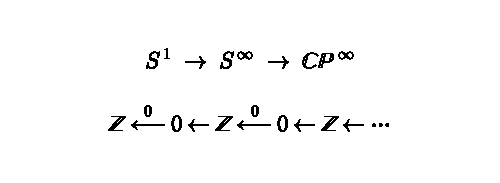
\includegraphics[width=0.5\textwidth,height=2.3in,keepaspectratio]{figs/cpinf.pdf}\end{center}
\begin{center}\renewcommand{\arraystretch}{1.25}\begin{tabular}{>{\raggedleft\arraybackslash}p{.17\textwidth}p{.68\textwidth}}\toprule
$\pi_1$ & $1$\\ $H_*$ & $H_{2k}=\mathbb{Z},\ \text{odd }0$\\ $\chi$ & $\text{undefined}$\\ \midrule
properties & \small compact: no; connected: yes; path-connected: yes; Hausdorff: yes; manifold: no; orientable: ---; simply connected: yes; contractible: no\\ \bottomrule\end{tabular}\end{center}
\pt{Method} Long exact sequence of $S^1\to S^\infty\to\mathbb{CP}^\infty$.
\pt{Sources} Not listed in the $\pi$-Base or in Steen and Seebach.
\subsection*{Point-set properties}
\pt{CW complex}One cell in each even dimension; not compact.
\subsection*{Algebraic invariants}
\pt{Homotopy}The fibration $S^1\to S^\infty\to\mathbb{CP}^\infty$ with contractible total space gives $\pi_k(\mathbb{CP}^\infty)\cong\pi_{k-1}(S^1)$: $\mathbb{Z}$ for $k=2$, zero otherwise.
\pt{Homology}Even cells only, so $H_{2k}=\mathbb{Z}$ for all $k\ge0$.
\pt{Line bundles}Homotopy classes $[X,\mathbb{CP}^\infty]$ correspond to $H^2(X;\mathbb{Z})$ and to isomorphism classes of complex line bundles on $X$, via the first Chern class.
\subsection*{Why it is in the zoo}Only one nonzero homotopy group, yet nonzero homology in every even degree. It classifies complex line bundles.
\pt{Where it appears} Circular coordinates for periodic data (\S\ref{app:app-circular}).
\bigskip
\entry{Dunce hat}{dunce}
\noindent$D$.\enspace A triangle with its three edges identified by the word $aaa^{-1}$.
\begin{center}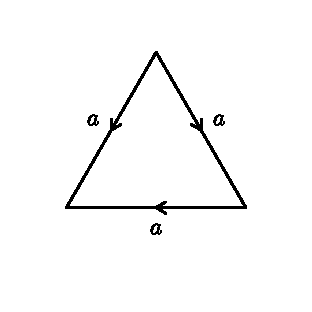
\includegraphics[width=0.5\textwidth,height=2.3in,keepaspectratio]{figs/dunce.pdf}\end{center}
\begin{center}\renewcommand{\arraystretch}{1.25}\begin{tabular}{>{\raggedleft\arraybackslash}p{.17\textwidth}p{.68\textwidth}}\toprule
$\pi_1$ & $1$\\ $H_*$ & $\mathbb{Z},\ 0,\ 0$\\ $\chi$ & $1$\\ \midrule
properties & \small compact: yes; connected: yes; path-connected: yes; Hausdorff: yes; manifold: no; orientable: ---; simply connected: yes; contractible: yes\\ \bottomrule\end{tabular}\end{center}
\pt{Method} $\pi_1=\langle a\mid aaa^{-1}\rangle=\langle a\mid a\rangle=1$, then Whitehead.
\pt{Sources} Not listed in the $\pi$-Base or in Steen and Seebach.
\subsection*{Point-set properties}
\pt{Compact, Hausdorff}Finite CW complex.
\pt{Not a manifold}The edge $a$ appears three times in the boundary of the triangle, so near a point of $a$ three half-disks meet along a line.
\subsection*{Algebraic invariants}
\pt{Cells}All corners are identified to one vertex. One $1$-cell $a$, one $2$-cell attached along $aaa^{-1}$.
\pt{Fundamental group}$\langle a\mid aaa^{-1}\rangle=\langle a\mid a\rangle=1$.
\pt{Homology}$\partial e=a+a-a=a$, so $d_2:\mathbb{Z}\to\mathbb{Z}$ is an isomorphism and $H_1=H_2=0$. $\chi=1-1+1=1$.
\pt{Contractible}Simply connected with $\tilde H_*=0$: Hurewicz gives $\pi_k=0$ for all $k$, and Whitehead gives contractibility.
\subsection*{Why it is in the zoo}Contractible but with no free face, so it cannot be simplicially collapsed. Bing's house with two rooms is the same phenomenon.
\bigskip
\entry{Hilbert cube}{hilbert}
\noindent$[0,1]^{\mathbb{N}}$.\enspace Countable product of intervals with the product topology; metrizable as $\prod[0,1/n]\subset\ell^2$.
\begin{center}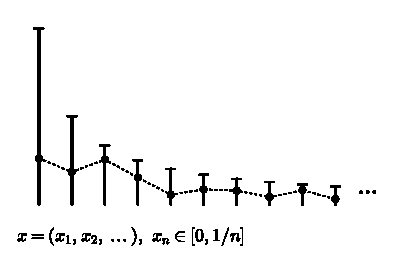
\includegraphics[width=0.5\textwidth,height=2.3in,keepaspectratio]{figs/hilbert.pdf}\end{center}
\begin{center}\renewcommand{\arraystretch}{1.25}\begin{tabular}{>{\raggedleft\arraybackslash}p{.17\textwidth}p{.68\textwidth}}\toprule
$\pi_1$ & $1$\\ $H_*$ & $\mathbb{Z},\ 0,\dots$\\ $\chi$ & $1$\\ \midrule
properties & \small compact: yes; connected: yes; path-connected: yes; Hausdorff: yes; manifold: no; orientable: ---; simply connected: yes; contractible: yes\\ \bottomrule\end{tabular}\end{center}
\pt{Method} Convex, so straight-line homotopy.
\pt{Sources} $\pi$-Base \href{https://topology.pi-base.org/spaces/S000032}{S000032}; Steen and Seebach, \emph{Counterexamples in Topology}, Example 38, p.~65.
\subsection*{Point-set properties}
\pt{Compact}Tychonoff's theorem; for a countable product of compact metric spaces a diagonal argument suffices.
\pt{Metrizable}$d(x,y)=\sum_n2^{-n}|x_n-y_n|$ induces the product topology.
\pt{Not a finite-dimensional manifold}It contains $[0,1]^n$ for every $n$ in every open set, so by invariance of domain no open set is homeomorphic to an open subset of $\mathbb{R}^m$.
\subsection*{Algebraic invariants}
\pt{Contractible}$H(x,t)=(1-t)x$ is continuous in the product topology.
\pt{Fixed points}Every continuous self-map has a fixed point (Schauder–Tychonoff).
\subsection*{Why it is in the zoo}Compact by Tychonoff, infinite-dimensional, homogeneous. Every compact metric space embeds in it.
\bigskip
\chapter{Pathological spaces}
\entry{Hawaiian earring}{hawaii}
\noindent$\mathbb{H}=\bigcup_n C_n$.\enspace Circles $C_n$ of radius $1/n$ centered at $(1/n,0)$, with the subspace topology from $\mathbb{R}^2$.
\begin{center}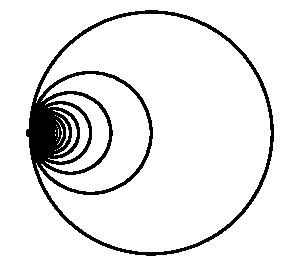
\includegraphics[width=0.5\textwidth,height=2.3in,keepaspectratio]{figs/hawaii.pdf}\end{center}
\begin{center}\renewcommand{\arraystretch}{1.25}\begin{tabular}{>{\raggedleft\arraybackslash}p{.17\textwidth}p{.68\textwidth}}\toprule
$\pi_1$ & $\text{uncountable, not free}$\\ $H_*$ & $\mathbb{Z},\ \text{uncountable},\dots$\\ $\chi$ & $\text{undefined}$\\ \midrule
properties & \small compact: yes; connected: yes; path-connected: yes; Hausdorff: yes; manifold: no; orientable: ---; simply connected: no; contractible: no\\ \bottomrule\end{tabular}\end{center}
\pt{Method} No clean method: van Kampen and covering space theory both fail at the origin.
\pt{Sources} $\pi$-Base \href{https://topology.pi-base.org/spaces/S000201}{S000201}.
\subsection*{Point-set properties}
\pt{Compact}Closed and bounded in $\mathbb{R}^2$. This is the difference from the CW wedge, whose topology is finer.
\pt{Not semilocally simply connected}Every neighborhood of the origin contains all $C_n$ for large $n$. The retraction $r_n:\mathbb{H}\to C_n$ that collapses the other circles shows $C_n$ is not null-homotopic in $\mathbb{H}$. So small loops at the origin are never trivial, and $\mathbb{H}$ has no simply connected cover.
\subsection*{Algebraic invariants}
\pt{Retractions}Collapsing $C_{n+1},C_{n+2},\dots$ retracts $\mathbb{H}$ onto the finite wedge $\bigvee_{i\le n}C_i$. These give compatible surjections $\pi_1(\mathbb{H})\to F_n$ and a homomorphism $\pi_1(\mathbb{H})\to\varprojlim F_n$, which is injective but not surjective.
\pt{Uncountable}A loop can run around $C_1$ in time $[0,\frac12]$, $C_2$ in $[\frac12,\frac34]$, and so on, and still be continuous at $t=1$ because the circles shrink. Choosing which circles to traverse gives $2^{\aleph_0}$ loops with distinct images in $\varprojlim F_n$.
\pt{Not free}Every finitely generated subgroup is free, but the whole group is not (Higman). $H_1$, the abelianization, is uncountable.
\subsection*{Why it is in the zoo}The standard example where computing $\pi_1$ is hard. It has no universal cover. Compare the infinite wedge of circles.
\bigskip
\entry{Warsaw circle}{warsaw}
\noindent$W$.\enspace The closed topologist's sine curve with its two ends joined by an arc.
\begin{center}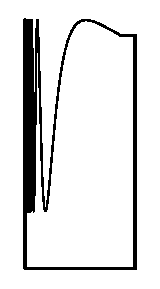
\includegraphics[width=0.5\textwidth,height=2.3in,keepaspectratio]{figs/warsaw.pdf}\end{center}
\begin{center}\renewcommand{\arraystretch}{1.25}\begin{tabular}{>{\raggedleft\arraybackslash}p{.17\textwidth}p{.68\textwidth}}\toprule
$\pi_1$ & $1$\\ $H_*$ & $\mathbb{Z},\ 0,\ 0,\dots$\\ $\chi$ & $1$\\ \midrule
properties & \small compact: yes; connected: yes; path-connected: yes; Hausdorff: yes; manifold: no; orientable: ---; simply connected: yes; contractible: no\\ \bottomrule\end{tabular}\end{center}
\pt{Method} A path cannot pass through the oscillating part, so every map of a sphere misses a point and lands in something contractible.
\pt{Sources} $\pi$-Base \href{https://topology.pi-base.org/spaces/S000205}{S000205}.
\subsection*{Point-set properties}
\pt{Compact, path-connected}Closed and bounded in $\mathbb{R}^2$. The extra arc joins the limit segment to the end of the curve, so it is path-connected, unlike the sine curve.
\pt{Not locally connected}Near a point of the limit segment, every small ball meets infinitely many separate pieces of the oscillating curve.
\subsection*{Algebraic invariants}
\pt{Paths cannot go around}No path travels from the limit segment into the oscillating curve, for the same reason the topologist's sine curve is not path-connected. So the compact image of any $S^k\to W$ omits some point $p$ of the oscillating part.
\pt{Weakly contractible}Each path component of $W\setminus\{p\}$ is contractible, and the image of a sphere lies in one of them, so every map $S^k\to W$ is null-homotopic. All $\pi_k(W)=0$, and the map to a point is a weak equivalence, so singular homology is that of a point.
\pt{Not contractible}$W$ is the intersection of nested annular neighborhoods, so its Čech cohomology is $\check H^1(W)=\varinjlim\check H^1(\text{annulus})=\mathbb{Z}$. Čech cohomology is a homotopy invariant and vanishes on contractible spaces.
\subsection*{Why it is in the zoo}All homotopy groups vanish but $W$ is not contractible, so Whitehead's theorem needs the CW hypothesis. Čech cohomology sees the circle: $\check H^1(W)\cong\mathbb{Z}$.
\bigskip
\entry{Topologist's sine curve}{sine}
\noindent$\overline{\{(x,\sin\tfrac1x):0<x\le1\}}$.\enspace The graph together with the limit segment $\{0\}\times[-1,1]$.
\begin{center}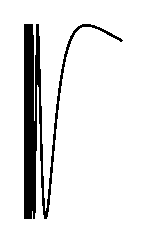
\includegraphics[width=0.5\textwidth,height=2.3in,keepaspectratio]{figs/sine.pdf}\end{center}
\begin{center}\renewcommand{\arraystretch}{1.25}\begin{tabular}{>{\raggedleft\arraybackslash}p{.17\textwidth}p{.68\textwidth}}\toprule
$\pi_1$ & $1\ \text{(each path component)}$\\ $H_*$ & $\mathbb{Z}^2,\ 0,\dots$\\ $\chi$ & $2$\\ \midrule
properties & \small compact: yes; connected: yes; path-connected: no; Hausdorff: yes; manifold: no; orientable: ---; simply connected: ---; contractible: no\\ \bottomrule\end{tabular}\end{center}
\pt{Method} Two path components, each contractible.
\pt{Sources} $\pi$-Base \href{https://topology.pi-base.org/spaces/S000114}{S000114}; Steen and Seebach, \emph{Counterexamples in Topology}, Example 117, p.~137.
\subsection*{Point-set properties}
\pt{Compact, connected}It is the closure of the graph, a connected set, and closures of connected sets are connected. Closed and bounded, so compact.
\pt{Not path-connected}Suppose $\gamma$ is a path from $(0,0)$ to a point of the graph. Let $t_0$ be the last time $\gamma$ is on the segment. Just after $t_0$ the $x$-coordinate is positive and tends to $0$, so the $y$-coordinate $\sin(1/x)$ takes both values $\pm1$ in every interval $(t_0,t_0+\delta)$. This contradicts continuity of $\gamma$ at $t_0$.
\subsection*{Algebraic invariants}
\pt{Homology}The path components are the graph $\cong(0,1]$ and the segment $\cong[-1,1]$, both contractible. Singular homology is the direct sum over path components: $H_0=\mathbb{Z}^2$, the rest zero. $\chi=2$.
\subsection*{Why it is in the zoo}Connected but not path-connected. Singular $H_0$ counts path components, not components.
\bigskip
\entry{Comb space}{comb}
\noindent$C$.\enspace The base $[0,1]\times\{0\}$ with vertical unit teeth at $x=0$ and at each $x=1/n$.
\begin{center}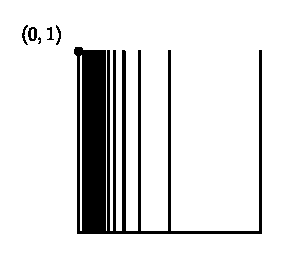
\includegraphics[width=0.5\textwidth,height=2.3in,keepaspectratio]{figs/comb.pdf}\end{center}
\begin{center}\renewcommand{\arraystretch}{1.25}\begin{tabular}{>{\raggedleft\arraybackslash}p{.17\textwidth}p{.68\textwidth}}\toprule
$\pi_1$ & $1$\\ $H_*$ & $\mathbb{Z},\ 0,\dots$\\ $\chi$ & $1$\\ \midrule
properties & \small compact: yes; connected: yes; path-connected: yes; Hausdorff: yes; manifold: no; orientable: ---; simply connected: yes; contractible: yes\\ \bottomrule\end{tabular}\end{center}
\pt{Method} Slide the teeth down to the base, then contract the base.
\pt{Sources} Not listed in the $\pi$-Base or in Steen and Seebach.
\subsection*{Point-set properties}
\pt{Compact}Closed and bounded: the teeth at $1/n$ accumulate on the tooth at $0$, which is included.
\pt{Not locally connected}A small ball around $(0,y)$ with $y>0$ meets infinitely many teeth in disjoint segments.
\subsection*{Algebraic invariants}
\pt{Contraction}First $H((x,y),t)=(x,(1-t)y)$ for $t\in[0,1]$, which slides every tooth down along itself; then contract $[0,1]\times\{0\}$ to a point.
\pt{No strong deformation retraction to $(0,1)$}During such a homotopy, points $(1/n,1)$ near $(0,1)$ must stay near $(0,1)$ for small times, but to reach it they must travel down their tooth and along the base. Continuity at $(0,1)$ fails.
\subsection*{Why it is in the zoo}Contractible but not locally connected, and it does not deformation retract onto $(0,1)$ while keeping that point fixed.
\bigskip
\entry{Dyadic solenoid}{solenoid}
\noindent$\Sigma_2=\varprojlim\big(S^1\xleftarrow{z^2}S^1\xleftarrow{z^2}\cdots\big)$.\enspace The inverse limit of circles under the doubling map; a compact connected abelian group.
\begin{center}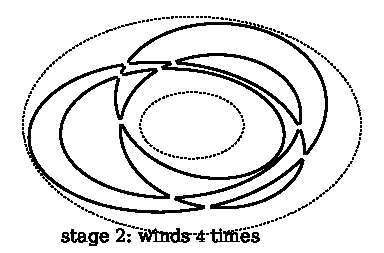
\includegraphics[width=0.5\textwidth,height=2.3in,keepaspectratio]{figs/solenoid.pdf}\end{center}
\begin{center}\renewcommand{\arraystretch}{1.25}\begin{tabular}{>{\raggedleft\arraybackslash}p{.17\textwidth}p{.68\textwidth}}\toprule
$\pi_1$ & $1\ \text{(each path component)}$\\ $H_*$ & $H_0\cong\bigoplus_{2^{\aleph_0}}\mathbb{Z}$\\ $\chi$ & $\text{undefined}$\\ \midrule
properties & \small compact: yes; connected: yes; path-connected: no; Hausdorff: yes; manifold: no; orientable: ---; simply connected: ---; contractible: no\\ \bottomrule\end{tabular}\end{center}
\pt{Method} Path components are dense continuous images of $\mathbb{R}$, uncountably many.
\pt{Sources} Not listed in the $\pi$-Base or in Steen and Seebach.
\subsection*{Point-set properties}
\pt{Compact, Hausdorff}A closed subset of the compact metrizable product $\prod S^1$.
\pt{Connected}An inverse limit of compact connected Hausdorff spaces is connected.
\pt{Locally a Cantor set times an interval}A small neighborhood looks like an arc times the 2-adic integers, so the space is not locally connected.
\subsection*{Algebraic invariants}
\pt{Path components}$t\mapsto(e^{2\pi it},e^{\pi it},e^{\pi it/2},\dots)$ maps $\mathbb{R}$ injectively onto the path component of the identity. The other path components are its cosets, and there are $2^{\aleph_0}$ of them.
\pt{Čech cohomology}Čech cohomology turns inverse limits of compact spaces into direct limits: $\check H^1(\Sigma_2)=\varinjlim(\mathbb{Z}\xrightarrow{2}\mathbb{Z}\xrightarrow{2}\cdots)=\mathbb{Z}[1/2]$.
\subsection*{Why it is in the zoo}Connected with uncountably many path components. Čech cohomology $\check H^1\cong\mathbb{Z}[1/2]$ records the inverse limit; singular theory does not.
\pt{Where it appears} Chaotic dynamics: the horseshoe and the solenoid (\S\ref{app:app-chaos}); Meter, polyrhythm, and phasing (\S\ref{app:app-rhythm}).
\bigskip
\entry{Cantor set}{cantor}
\noindent$C\cong\{0,1\}^{\mathbb{N}}$.\enspace Middle thirds removed from $[0,1]$, forever.
\begin{center}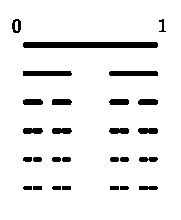
\includegraphics[width=0.5\textwidth,height=2.3in,keepaspectratio]{figs/cantor.pdf}\end{center}
\begin{center}\renewcommand{\arraystretch}{1.25}\begin{tabular}{>{\raggedleft\arraybackslash}p{.17\textwidth}p{.68\textwidth}}\toprule
$\pi_1$ & $1\ \text{(at each point)}$\\ $H_*$ & $H_0\cong\bigoplus_{2^{\aleph_0}}\mathbb{Z}$\\ $\chi$ & $\text{undefined}$\\ \midrule
properties & \small compact: yes; connected: no; path-connected: no; Hausdorff: yes; manifold: no; orientable: ---; simply connected: ---; contractible: no\\ \bottomrule\end{tabular}\end{center}
\pt{Method} Totally disconnected, so every path is constant.
\pt{Sources} $\pi$-Base \href{https://topology.pi-base.org/spaces/S000026}{S000026}; Steen and Seebach, \emph{Counterexamples in Topology}, Example 29, p.~57.
\subsection*{Point-set properties}
\pt{Compact}An intersection of closed subsets of $[0,1]$.
\pt{Totally disconnected}Between two points of $C$ there is a removed open interval. Splitting at it writes $C$ as a union of two disjoint clopen sets separating the points.
\pt{Perfect}Every point is a limit of endpoints of the construction.
\pt{Product model}Ternary expansions with digits $0,2$ give a homeomorphism $C\to\{0,2\}^{\mathbb{N}}$.
\subsection*{Algebraic invariants}
\pt{Homology}A path has connected image, which must be a point. Singular simplices are constant, so the chain complex is a direct sum of copies of that of a point, one for each element of $C$.
\subsection*{Why it is in the zoo}Compact, perfect, totally disconnected, and metrizable. Every compact metric space is a continuous image of it.
\pt{Where it appears} Chaotic dynamics: the horseshoe and the solenoid (\S\ref{app:app-chaos}).
\bigskip
\entry{Long line}{longline}
\noindent$L=\omega_1\times[0,1)$.\enspace Uncountably many unit intervals glued end to end, with the lexicographic order topology.
\begin{center}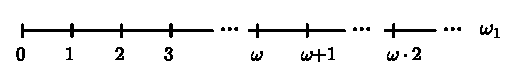
\includegraphics[width=0.5\textwidth,height=2.3in,keepaspectratio]{figs/longline.pdf}\end{center}
\begin{center}\renewcommand{\arraystretch}{1.25}\begin{tabular}{>{\raggedleft\arraybackslash}p{.17\textwidth}p{.68\textwidth}}\toprule
$\pi_1$ & $1$\\ $H_*$ & $\mathbb{Z},\ 0,\dots$\\ $\chi$ & $1$\\ \midrule
properties & \small compact: no; connected: yes; path-connected: yes; Hausdorff: yes; manifold: no; orientable: ---; simply connected: yes; contractible: no\\ \bottomrule\end{tabular}\end{center}
\pt{Method} Every compact subset lies in a countable initial segment, which is an interval.
\pt{Sources} $\pi$-Base \href{https://topology.pi-base.org/spaces/S000038}{S000038}; Steen and Seebach, \emph{Counterexamples in Topology}, Example 45, p.~71.
\subsection*{Point-set properties}
\pt{Connected}A linearly ordered set with the least upper bound property and no gaps is connected in the order topology.
\pt{Locally Euclidean, not second countable}Each point has a neighborhood order-isomorphic to an open interval. The open intervals $(\alpha\times\{\frac12\},(\alpha+1)\times\{\frac12\})$ form an uncountable disjoint family, which a countable base cannot accommodate.
\pt{Not compact, not metrizable}It is sequentially compact, since every countable set is bounded, but not compact: the initial segments cover it with no finite subcover. A metric space that is sequentially compact is compact, so $L$ is not metrizable.
\subsection*{Algebraic invariants}
\pt{Homotopy groups}A countable ordinal $\alpha$ gives an initial segment $[0,\alpha]\cong[0,1]$. Every compact image of a sphere lies in such a segment, so it is null-homotopic.
\pt{Not contractible}A contraction would be a homotopy $L\times[0,1]\to L$. An argument with closed unbounded subsets of $\omega_1$ shows this is impossible.
\subsection*{Why it is in the zoo}Locally Euclidean and Hausdorff but not second countable. All homotopy groups vanish, yet it is not contractible.
\bigskip
\entry{Rationals}{rationals}
\noindent$\mathbb{Q}$.\enspace Subspace topology from $\mathbb{R}$.
\begin{center}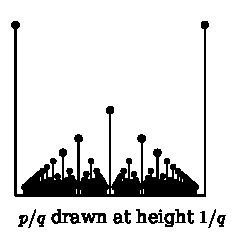
\includegraphics[width=0.5\textwidth,height=2.3in,keepaspectratio]{figs/rationals.pdf}\end{center}
\begin{center}\renewcommand{\arraystretch}{1.25}\begin{tabular}{>{\raggedleft\arraybackslash}p{.17\textwidth}p{.68\textwidth}}\toprule
$\pi_1$ & $1\ \text{(at each point)}$\\ $H_*$ & $H_0\cong\bigoplus_{\mathbb{N}}\mathbb{Z}$\\ $\chi$ & $\text{undefined}$\\ \midrule
properties & \small compact: no; connected: no; path-connected: no; Hausdorff: yes; manifold: no; orientable: ---; simply connected: ---; contractible: no\\ \bottomrule\end{tabular}\end{center}
\pt{Method} Totally disconnected.
\pt{Sources} $\pi$-Base \href{https://topology.pi-base.org/spaces/S000027}{S000027}; Steen and Seebach, \emph{Counterexamples in Topology}, Example 30, p.~59.
\subsection*{Point-set properties}
\pt{Totally disconnected}For rationals $p<q$ pick an irrational $r$ between them; $(-\infty,r)\cap\mathbb{Q}$ is clopen.
\pt{Not locally compact}The closure in $\mathbb{Q}$ of any interval $(a,b)\cap\mathbb{Q}$ contains sequences converging to irrationals, which have no convergent subsequence in $\mathbb{Q}$.
\subsection*{Algebraic invariants}
\pt{Homology}Paths are constant, so $H_0$ is free on the countably many points and the rest vanishes.
\subsection*{Why it is in the zoo}Not locally compact. Every countable metric space with no isolated points is homeomorphic to $\mathbb{Q}$ (Sierpiński).
\bigskip
\entry{Sorgenfrey line}{sorgenfrey}
\noindent$\mathbb{R}_\ell$.\enspace $\mathbb{R}$ with basis the half-open intervals $[a,b)$.
\begin{center}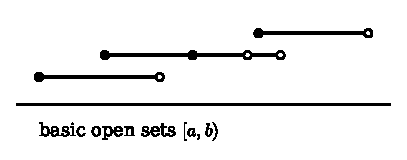
\includegraphics[width=0.5\textwidth,height=2.3in,keepaspectratio]{figs/sorgenfrey.pdf}\end{center}
\begin{center}\renewcommand{\arraystretch}{1.25}\begin{tabular}{>{\raggedleft\arraybackslash}p{.17\textwidth}p{.68\textwidth}}\toprule
$\pi_1$ & $1\ \text{(at each point)}$\\ $H_*$ & $H_0\cong\bigoplus_{2^{\aleph_0}}\mathbb{Z}$\\ $\chi$ & $\text{undefined}$\\ \midrule
properties & \small compact: no; connected: no; path-connected: no; Hausdorff: yes; manifold: no; orientable: ---; simply connected: ---; contractible: no\\ \bottomrule\end{tabular}\end{center}
\pt{Method} Totally disconnected: $[a,b)$ is clopen.
\pt{Sources} $\pi$-Base \href{https://topology.pi-base.org/spaces/S000043}{S000043}; Steen and Seebach, \emph{Counterexamples in Topology}, Example 51, p.~75.
\subsection*{Point-set properties}
\pt{Totally disconnected}$[a,b)$ is open, and its complement $(-\infty,a)\cup[b,\infty)$ is a union of basic sets, so $[a,b)$ is also closed.
\pt{Countability}$\mathbb{Q}$ is dense and $[x,x+\frac1n)$ is a countable local base. Any base must contain, for each $x$, a set with minimum $x$, so it is uncountable.
\pt{The Sorgenfrey plane}The antidiagonal $\{(x,-x)\}$ is closed and discrete in $\mathbb{R}_\ell^2$ and has size $2^{\aleph_0}$. Jones' lemma then shows the separable space $\mathbb{R}_\ell^2$ is not normal.
\subsection*{Algebraic invariants}
\pt{Homology}Connected subsets are points, so paths are constant and $H_0$ is free on $2^{\aleph_0}$ generators.
\subsection*{Why it is in the zoo}Normal and Lindelöf, but $\mathbb{R}_\ell\times\mathbb{R}_\ell$ is not normal. Separable and first countable but not second countable.
\bigskip
\chapter{Non-Hausdorff and finite spaces}
\entry{Line with two origins}{twoorigins}
\noindent$\mathbb{R}\sqcup\mathbb{R}/(x\sim x,\ x\ne0)$.\enspace Two copies of $\mathbb{R}$ glued everywhere except at $0$.
\begin{center}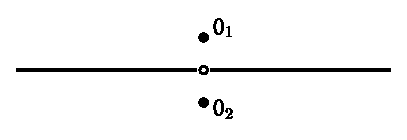
\includegraphics[width=0.5\textwidth,height=2.3in,keepaspectratio]{figs/twoorigins.pdf}\end{center}
\begin{center}\renewcommand{\arraystretch}{1.25}\begin{tabular}{>{\raggedleft\arraybackslash}p{.17\textwidth}p{.68\textwidth}}\toprule
$\pi_1$ & $\mathbb{Z}$\\ $H_*$ & $\mathbb{Z},\ \mathbb{Z},\ 0$\\ $\chi$ & $0$\\ \midrule
properties & \small compact: no; connected: yes; path-connected: yes; Hausdorff: no; manifold: no; orientable: ---; simply connected: no; contractible: no\\ \bottomrule\end{tabular}\end{center}
\pt{Method} The two copies of $\mathbb{R}$ overlap in two pieces, which creates a loop.
\pt{Sources} $\pi$-Base \href{https://topology.pi-base.org/spaces/S000083}{S000083}.
\subsection*{Point-set properties}
\pt{Locally Euclidean, second countable}Each copy of $\mathbb{R}$ is open and is a chart.
\pt{Not Hausdorff}Every neighborhood of $0_1$ and every neighborhood of $0_2$ contain $(-\varepsilon,\varepsilon)\setminus\{0\}$ for some $\varepsilon$, so they meet.
\subsection*{Algebraic invariants}
\pt{A loop}Go from $1$ to $0_1$ to $-1$ in the first copy, then from $-1$ to $0_2$ to $1$ in the second copy. This loop is not null-homotopic.
\pt{Mayer–Vietoris}Use $U,V$ the two copies, each contractible, with $U\cap V=\mathbb{R}\setminus\{0\}$, two contractible pieces. Mayer–Vietoris holds for open covers of any space: $0\to H_1(X)\to H_0(U\cap V)$ $\to H_0(U)\oplus H_0(V)\to H_0(X)\to0$, where $H_0(U\cap V)=\mathbb{Z}^2$ and $H_0(U)\oplus H_0(V)=\mathbb{Z}^2$. The middle map is $(x,y)\mapsto(x+y,-x-y)$, with kernel $\mathbb{Z}$. So $H_1=\mathbb{Z}$.
\pt{Fundamental group}The groupoid form of van Kampen gives $\pi_1=\mathbb{Z}$; the space is weakly equivalent to $S^1$.
\subsection*{Why it is in the zoo}Locally Euclidean and second countable; only Hausdorff fails, and that alone produces $\pi_1\cong\mathbb{Z}$.
\bigskip
\entry{Pseudocircle}{pseudocircle}
\noindent$\mathbb{S}=\{a,b,c,d\}$.\enspace Four points; open sets generated by $\{a\},\{b\},\{a,b,c\},\{a,b,d\}$.
\begin{center}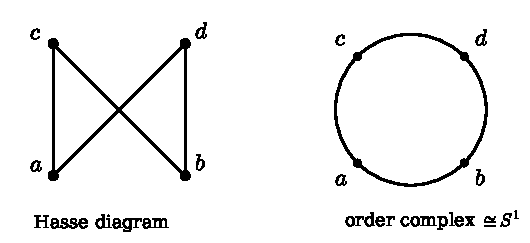
\includegraphics[width=0.82\textwidth,height=2.3in,keepaspectratio]{figs/pseudocircle.pdf}\end{center}
\begin{center}\renewcommand{\arraystretch}{1.25}\begin{tabular}{>{\raggedleft\arraybackslash}p{.17\textwidth}p{.68\textwidth}}\toprule
$\pi_1$ & $\mathbb{Z}$\\ $H_*$ & $\mathbb{Z},\ \mathbb{Z},\ 0$\\ $\chi$ & $0$\\ \midrule
properties & \small compact: yes; connected: yes; path-connected: yes; Hausdorff: no; manifold: no; orientable: ---; simply connected: no; contractible: no\\ \bottomrule\end{tabular}\end{center}
\pt{Method} McCord: a finite $T_0$ space is weakly equivalent to the order complex of its poset, here a 4-cycle.
\pt{Sources} $\pi$-Base \href{https://topology.pi-base.org/spaces/S000213}{S000213}.
\subsection*{Point-set properties}
\pt{Path-connected}$\gamma(0)=c$, $\gamma(t)=a$ for $t>0$ is continuous: the preimage of each open set is $\emptyset$, $(0,1]$, or $[0,1]$. Similar paths join every pair of points.
\pt{$T_0$, not $T_1$}$\{a\}$ is not closed, since its complement $\{b,c,d\}$ is not open. Distinct points are distinguished by some open set.
\subsection*{Algebraic invariants}
\pt{Van Kampen picture}$U=\{a,b,c\}$ and $V=\{a,b,d\}$ are open and contractible (each contracts onto its closed point $c$ or $d$). $U\cap V=\{a,b\}$ is discrete with two points. This is the same pattern as the line with two origins, so $\pi_1=\mathbb{Z}$ and $H_1=\mathbb{Z}$.
\pt{Order complex}The specialization order has $a,b<c$ and $a,b<d$. The order complex has vertices $a,b,c,d$ and edges $ac,ad,bc,bd$, a square, which is a circle.
\subsection*{Why it is in the zoo}A four-point space with $\pi_1\cong\mathbb{Z}$. Every finite simplicial complex is weakly equivalent to a finite space.
\pt{Where it appears} Digital topology and finite spaces (\S\ref{app:app-digital}).
\bigskip
\entry{Sierpiński space}{sierpinski}
\noindent$\{0,1\},\ \text{open sets }\emptyset,\{1\},\{0,1\}$.\enspace Two points, one open and one closed.
\begin{center}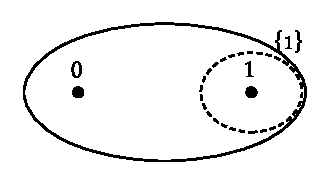
\includegraphics[width=0.5\textwidth,height=2.3in,keepaspectratio]{figs/sierpinski.pdf}\end{center}
\begin{center}\renewcommand{\arraystretch}{1.25}\begin{tabular}{>{\raggedleft\arraybackslash}p{.17\textwidth}p{.68\textwidth}}\toprule
$\pi_1$ & $1$\\ $H_*$ & $\mathbb{Z},\ 0,\dots$\\ $\chi$ & $1$\\ \midrule
properties & \small compact: yes; connected: yes; path-connected: yes; Hausdorff: no; manifold: no; orientable: ---; simply connected: yes; contractible: yes\\ \bottomrule\end{tabular}\end{center}
\pt{Method} Contract everything to the open point at once.
\pt{Sources} $\pi$-Base \href{https://topology.pi-base.org/spaces/S000010}{S000010}; Steen and Seebach, \emph{Counterexamples in Topology}, Example 11, p.~44.
\subsection*{Point-set properties}
\pt{Not $T_1$}$\{1\}$ is not closed.
\pt{Classifies open sets}$f:X\to\{0,1\}$ is continuous iff $f^{-1}(1)$ is open.
\subsection*{Algebraic invariants}
\pt{Contraction}$H(x,0)=x$ and $H(x,t)=1$ for $t>0$. The preimage of $\{1\}$ is $(\{0,1\}\times(0,1])\cup(\{1\}\times[0,1])$, which is open, so $H$ is continuous.
\subsection*{Why it is in the zoo}$T_0$ but not $T_1$. Continuous maps from $X$ to it correspond to open subsets of $X$.
\pt{Where it appears} Observable properties and the Sierpiński space (\S\ref{app:app-observable}); Digital topology and finite spaces (\S\ref{app:app-digital}).
\bigskip
\entry{Countable cofinite space}{cofinite}
\noindent$(\mathbb{N},\ \text{cofinite})$.\enspace Open sets are $\emptyset$ and complements of finite sets.
\begin{center}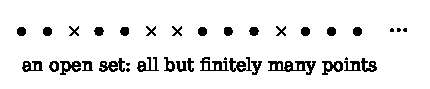
\includegraphics[width=0.5\textwidth,height=2.3in,keepaspectratio]{figs/cofinite.pdf}\end{center}
\begin{center}\renewcommand{\arraystretch}{1.25}\begin{tabular}{>{\raggedleft\arraybackslash}p{.17\textwidth}p{.68\textwidth}}\toprule
$\pi_1$ & $1\ \text{(at each point)}$\\ $H_*$ & $H_0\cong\bigoplus_{\mathbb{N}}\mathbb{Z}$\\ $\chi$ & $\text{undefined}$\\ \midrule
properties & \small compact: yes; connected: yes; path-connected: no; Hausdorff: no; manifold: no; orientable: ---; simply connected: ---; contractible: no\\ \bottomrule\end{tabular}\end{center}
\pt{Method} Sierpiński's theorem forces every path to be constant.
\pt{Sources} $\pi$-Base \href{https://topology.pi-base.org/spaces/S000015}{S000015}; Steen and Seebach, \emph{Counterexamples in Topology}, Example 18, p.~49.
\subsection*{Point-set properties}
\pt{Compact}Any nonempty open set misses only finitely many points, which finitely many more sets cover.
\pt{$T_1$, not Hausdorff, connected}Points are closed. Two nonempty open sets have finite complements in an infinite set, so they intersect; in particular no separation exists.
\pt{Not path-connected}For a path $\gamma:[0,1]\to\mathbb{N}$, the fibers $\gamma^{-1}(n)$ are disjoint closed sets covering $[0,1]$, countably many. Sierpiński's theorem: a compact connected Hausdorff space is not a countable union of two or more disjoint nonempty closed sets. So one fiber is everything and $\gamma$ is constant.
\pt{Uncountable case}On $\mathbb{R}$, any injection $[0,1]\to\mathbb{R}$ is continuous for the cofinite topology, since preimages of finite sets are finite and hence closed.
\subsection*{Algebraic invariants}
\pt{Homology}Paths are constant, so $H_0$ is free on the points and the rest vanishes.
\subsection*{Why it is in the zoo}$T_1$, compact, connected, but not path-connected. On an uncountable set such as $\mathbb{R}$ the cofinite topology is path-connected.
\pt{Where it appears} Observable properties and the Sierpiński space (\S\ref{app:app-observable}); The Zariski topology of a curve (\S\ref{app:app-zariski}).
\bigskip
\chapter{Why we care: applications}
The spaces in this zoo were not invented for their own sake. Each section below names a problem from physics, data analysis, music theory, engineering, or economics, the spaces it uses, and the invariant that does the work, with references back to the entries where those invariants are derived.
\section{Physics}
\subsection{Spin one-half and the belt trick}\label{app:app-spin}
\noindent\textit{Spaces:} Rotation group (\S\ref{sp:so3}), Sphere (\S\ref{sp:sphere}).\enspace\textit{Invariant:} $\pi_1(SO(3))=\mathbb{Z}/2$.

Quantum states only need to be defined up to a phase, so a rotation can act on a state through the universal cover $SU(2)\cong S^3$ instead of through $SO(3)$ itself. Because $\pi_1(SO(3))$ has order two, there are exactly two possibilities: a rotation by $2\pi$ acts as $+1$ (integer spin) or as $-1$ (half-integer spin). Electrons, protons, and neutrons are of the second kind. The sign change was observed directly in 1975 by sending neutrons through an interferometer, rotating the spin on one arm by $2\pi$, and watching the interference pattern invert; a rotation by $4\pi$ restores it. The belt trick is the same fact for a physical belt: a $2\pi$ twist cannot be undone without rotating the buckle, a $4\pi$ twist can.
\begin{list}{}{\leftmargin=1.2em\itemindent=-1.2em\itemsep=0pt}\small \item H. Rauch et al., Verification of coherent spinor rotation of fermions, Physics Letters A 54 (1975) 425.\item S. A. Werner et al., Observation of the phase shift of a neutron due to precession in a magnetic field, Phys. Rev. Lett. 35 (1975) 1053.\end{list}
\subsection{The Aharonov–Bohm effect}\label{app:app-ab}
\noindent\textit{Spaces:} Wedge of n circles (\S\ref{sp:rose}), Annulus and solid torus (\S\ref{sp:annulus}), Circle (\S\ref{sp:circle}).\enspace\textit{Invariant:} $\pi_1(\mathbb{R}^2\setminus\{0\})=\mathbb{Z}$.

\begin{center}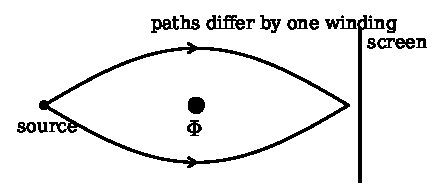
\includegraphics[width=0.55\textwidth,height=2.6in,keepaspectratio]{figs/app_ab.pdf}\end{center}
A long shielded solenoid confines its magnetic field to a thin tube, so electrons moving around it travel through a region where the field is zero. That region is the plane minus a disk, which deformation retracts onto a circle. Each path an electron can take has a winding number around the solenoid, and the quantum phase it picks up is $e^{iq\Phi n/\hbar}$, where $\Phi$ is the enclosed flux and $n$ the winding number. Two beams passing on opposite sides differ by one winding, so their interference pattern shifts with $\Phi$ even though no force acts on either beam. The effect is measurable precisely because the field-free region is not simply connected: in a simply connected region, a field-free potential could be gauged away entirely.
\begin{list}{}{\leftmargin=1.2em\itemindent=-1.2em\itemsep=0pt}\small \item Y. Aharonov and D. Bohm, Significance of electromagnetic potentials in the quantum theory, Phys. Rev. 115 (1959) 485.\end{list}
\subsection{Anyons and braid statistics}\label{app:app-anyons}
\noindent\textit{Spaces:} Configuration space (\S\ref{sp:conf}), Finite connected graph (\S\ref{sp:graph}).\enspace\textit{Invariant:} $\pi_1(\mathrm{UConf}_n(\mathbb{C}))=B_n$.

The configuration space of $n$ identical particles is the space of unordered $n$-point subsets. Exchanging particles traces a loop in it, and the quantum state picks up a phase determined by a one-dimensional representation of its fundamental group. In three dimensions the diagonals have codimension three, the fundamental group is the symmetric group $S_n$, and the only one-dimensional representations give bosons ($+1$) and fermions ($-1$). In the plane the fundamental group is the braid group $B_n$, whose abelianization is $\mathbb{Z}$, so any phase $e^{i\theta}$ can occur. These intermediate particles, anyons, describe excitations of fractional quantum Hall systems, and non-abelian versions are the basis of proposals for topological quantum computing.
\begin{list}{}{\leftmargin=1.2em\itemindent=-1.2em\itemsep=0pt}\small \item J. M. Leinaas and J. Myrheim, On the theory of identical particles, Il Nuovo Cimento B 37 (1977) 1.\item F. Wilczek, Quantum mechanics of fractional-spin particles, Phys. Rev. Lett. 49 (1982) 957.\end{list}
\subsection{Topological defects in ordered media}\label{app:app-defects}
\noindent\textit{Spaces:} Circle (\S\ref{sp:circle}), Real projective plane (\S\ref{sp:rp2}), Sphere (\S\ref{sp:sphere}).\enspace\textit{Invariant:} $\pi_1(S^1)=\mathbb{Z},\ \ \pi_1(\mathbb{RP}^2)=\mathbb{Z}/2,\ \ \pi_2(S^2)=\mathbb{Z}$.

\begin{center}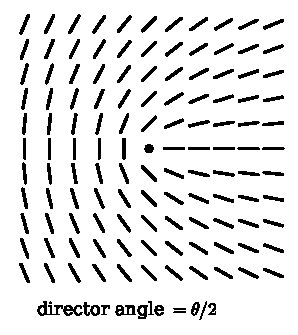
\includegraphics[width=0.55\textwidth,height=2.6in,keepaspectratio]{figs/app_nematic.pdf}\end{center}
An ordered medium assigns to each point a value in an order parameter space $M$. Around a line defect the order parameter traces a loop in $M$, so line defects are classified by $\pi_1(M)$, and point defects in three dimensions by $\pi_2(M)$. In superfluid helium the order parameter is a phase in $S^1$, and $\pi_1=\mathbb{Z}$ means vortices carry an integer winding number. In a nematic liquid crystal the molecules are rods with no head or tail, so the order parameter is a line through the origin, a point of $\mathbb{RP}^2$. Since $\pi_1(\mathbb{RP}^2)=\mathbb{Z}/2$, there is exactly one kind of stable line defect, the half-integer disclination, and two of them can annihilate. Point defects (hedgehogs) are classified by $\pi_2(\mathbb{RP}^2)=\mathbb{Z}$.
\begin{list}{}{\leftmargin=1.2em\itemindent=-1.2em\itemsep=0pt}\small \item N. D. Mermin, The topological theory of defects in ordered media, Rev. Mod. Phys. 51 (1979) 591.\end{list}
\subsection{The Dirac monopole and charge quantization}\label{app:app-monopole}
\noindent\textit{Spaces:} Sphere (\S\ref{sp:sphere}), Complex projective space (\S\ref{sp:cpn}), Unitary group (\S\ref{sp:un}).\enspace\textit{Invariant:} $\pi_1(U(1))=\mathbb{Z}$.

A magnetic monopole would have a field on the sphere surrounding it that cannot be written with a single vector potential. Instead one uses two potentials on the northern and southern hemispheres, related on the equator by a gauge transformation $S^1\to U(1)$. For the electron's wavefunction to be single-valued, this transition function must be a closed loop in $U(1)$, which has a winding number in $\pi_1(U(1))=\mathbb{Z}$. The result is Dirac's condition that electric charge times magnetic charge is an integer multiple of a fixed constant. Geometrically, the monopole is a circle bundle over $S^2$, and the one with winding number one is the Hopf fibration $S^3\to S^2=\mathbb{CP}^1$.
\begin{list}{}{\leftmargin=1.2em\itemindent=-1.2em\itemsep=0pt}\small \item P. A. M. Dirac, Quantised singularities in the electromagnetic field, Proc. Roy. Soc. A 133 (1931) 60.\end{list}
\subsection{Instantons and the vacuum of gauge theory}\label{app:app-instanton}
\noindent\textit{Spaces:} Sphere (\S\ref{sp:sphere}), Unitary group (\S\ref{sp:un}), Rotation group (\S\ref{sp:so3}).\enspace\textit{Invariant:} $\pi_3(SU(2))=\pi_3(S^3)=\mathbb{Z}$.

In Euclidean $SU(2)$ Yang–Mills theory, a finite-action field must approach a pure gauge at infinity. The sphere at infinity in $\mathbb{R}^4$ is $S^3$, so the boundary data is a map $S^3\to SU(2)\cong S^3$, which has an integer degree. This degree is the instanton number. Configurations with different degrees cannot be deformed into each other, which splits the vacuum into sectors labeled by integers and leads to the $\theta$-parameter of QCD. The same group $\pi_3(S^3)=\mathbb{Z}$ appears in the sphere entry as the statement that $\pi_n(S^n)=\mathbb{Z}$.
\begin{list}{}{\leftmargin=1.2em\itemindent=-1.2em\itemsep=0pt}\small \item A. A. Belavin, A. M. Polyakov, A. S. Schwartz, Yu. S. Tyupkin, Pseudoparticle solutions of the Yang–Mills equations, Phys. Lett. B 59 (1975) 85.\end{list}
\subsection{The quantum Hall effect and Chern numbers}\label{app:app-hall}
\noindent\textit{Spaces:} Torus (\S\ref{sp:torus}), n-torus (\S\ref{sp:ntorus}), Complex projective space (\S\ref{sp:cpn}).\enspace\textit{Invariant:} $c_1\in H^2(T^2;\mathbb{Z})=\mathbb{Z}$.

Electron momenta in a two-dimensional crystal are periodic in both directions, so the space of momenta, the Brillouin zone, is a torus $T^2$. Each filled energy band gives a line bundle over this torus, a map $T^2\to\mathbb{CP}^\infty$ up to homotopy, and such a bundle has an integer invariant, the first Chern number. Thouless, Kohmoto, Nightingale, and den Nijs showed that the Hall conductance equals $e^2/h$ times the sum of these integers. This explains why the measured conductance sits on plateaus at exact integer multiples, to parts per billion, regardless of impurities in the sample. Topological insulators extend the same idea to other classes of bundles.
\begin{list}{}{\leftmargin=1.2em\itemindent=-1.2em\itemsep=0pt}\small \item D. J. Thouless, M. Kohmoto, M. P. Nightingale, M. den Nijs, Quantized Hall conductance in a two-dimensional periodic potential, Phys. Rev. Lett. 49 (1982) 405.\end{list}
\subsection{Qubits, the Bloch sphere, and geometric phase}\label{app:app-bloch}
\noindent\textit{Spaces:} Complex projective space (\S\ref{sp:cpn}), Sphere (\S\ref{sp:sphere}).\enspace\textit{Invariant:} $\{\text{pure states of }\mathbb{C}^n\}=\mathbb{CP}^{n-1}$.

A quantum state is a unit vector up to a phase, so the pure states of an $n$-level system form $\mathbb{CP}^{n-1}$. For a qubit this is $\mathbb{CP}^1\cong S^2$, the Bloch sphere used throughout quantum computing. When a spin-one-half system is carried slowly around a closed loop on this sphere, it returns with an extra phase equal to minus half the solid angle the loop encloses. This geometric (Berry) phase depends only on the path in $\mathbb{CP}^1$, not on how fast it is traversed, and it is the holonomy of the Hopf bundle $S^3\to S^2$.
\begin{list}{}{\leftmargin=1.2em\itemindent=-1.2em\itemsep=0pt}\small \item M. V. Berry, Quantal phase factors accompanying adiabatic changes, Proc. Roy. Soc. A 392 (1984) 45.\end{list}
\subsection{The toric code}\label{app:app-toric}
\noindent\textit{Spaces:} Torus (\S\ref{sp:torus}), Orientable surface of genus g (\S\ref{sp:genusg}).\enspace\textit{Invariant:} $H_1(\Sigma_g;\mathbb{Z}/2)=(\mathbb{Z}/2)^{2g}$.

\begin{center}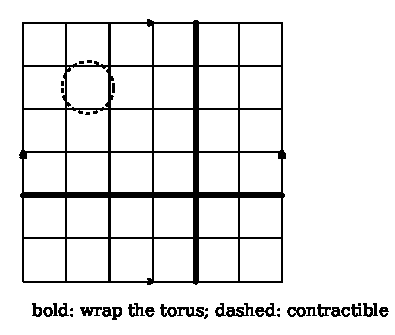
\includegraphics[width=0.55\textwidth,height=2.6in,keepaspectratio]{figs/app_toric.pdf}\end{center}
Kitaev's toric code places qubits on the edges of a square lattice drawn on a torus. Its ground states are labeled by $H_1(T^2;\mathbb{Z}/2)=(\mathbb{Z}/2)^2$, so there are four of them, and they store two logical qubits. A logical operation is a string of flips along a loop that wraps the torus; a contractible loop does nothing. Local noise produces short strings that bound small regions, which can be detected and corrected, while changing the stored information requires an error chain that wraps all the way around. On a surface of genus $g$ the code stores $2g$ qubits. This homological idea underlies the surface codes used in current quantum error-correction experiments.
\begin{list}{}{\leftmargin=1.2em\itemindent=-1.2em\itemsep=0pt}\small \item A. Yu. Kitaev, Fault-tolerant quantum computation by anyons, Annals of Physics 303 (2003) 2.\end{list}
\subsection{The shape of the universe}\label{app:app-cosmic}
\noindent\textit{Spaces:} Poincaré homology sphere (\S\ref{sp:poincare}), n-torus (\S\ref{sp:ntorus}), Lens space (\S\ref{sp:lens}).\enspace\textit{Invariant:} $\pi_1\ \text{finite}\Rightarrow\text{multiple images}$.

General relativity fixes the local geometry of space but not its global topology. If space were a quotient of $S^3$ or $\mathbb{R}^3$ by a group of isometries, light could reach us along several paths, and the cosmic microwave background would contain pairs of matching circles. In 2003 Luminet and collaborators proposed that space is the Poincaré homology sphere, a dodecahedron with opposite faces glued, to explain the unusually weak large-angle correlations seen by WMAP. Later searches for matching circles, including with Planck data, found no such signal, and the proposal is now disfavored. The example shows how a quotient $S^3/\pi_1$ makes a concrete, testable prediction.
\begin{list}{}{\leftmargin=1.2em\itemindent=-1.2em\itemsep=0pt}\small \item J.-P. Luminet, J. R. Weeks, A. Riazuelo, R. Lehoucq, J.-P. Uzan, Dodecahedral space topology as an explanation for weak wide-angle temperature correlations in the cosmic microwave background, Nature 425 (2003) 593. \url{https://arxiv.org/abs/astro-ph/0310253}\end{list}
\subsection{Chaotic dynamics: the horseshoe and the solenoid}\label{app:app-chaos}
\noindent\textit{Spaces:} Cantor set (\S\ref{sp:cantor}), Dyadic solenoid (\S\ref{sp:solenoid}), Annulus and solid torus (\S\ref{sp:annulus}).\enspace\textit{Invariant:} $\Lambda\cong\{0,1\}^{\mathbb{Z}}$.

Smale's horseshoe stretches a square, folds it, and lays it back over itself. The points that stay in the square forever form a Cantor set, and on it the map is the shift on two-sided sequences of $0$s and $1$s, so the dynamics contains periodic orbits of every period and orbits that are dense. The solenoid arises the same way from a solid torus: stretch it to twice its length, thin it, and wrap it twice around inside itself. The intersection of all the images is the dyadic solenoid, a compact attractor that is locally a Cantor set times an interval. Both spaces enter dynamics as invariant sets that a computer simulation shows only as a blur.
\begin{list}{}{\leftmargin=1.2em\itemindent=-1.2em\itemsep=0pt}\small \item S. Smale, Differentiable dynamical systems, Bull. Amer. Math. Soc. 73 (1967) 747.\end{list}
\section{Data, images, and the brain}
\subsection{A Klein bottle in natural images}\label{app:app-klein}
\noindent\textit{Spaces:} Klein bottle (\S\ref{sp:klein}), Circle (\S\ref{sp:circle}).\enspace\textit{Invariant:} $H_*(\,\cdot\,;\mathbb{Z}/2)\ \text{of a point cloud}$.

Carlsson, Ishkhanov, de Silva, and Zomorodian took millions of $3\times3$ pixel patches from photographs, kept the high-contrast ones, and normalized them to points on a 7-sphere. Persistent homology of the densest region showed a circle: patches that look like an edge at some angle. A larger region showed a space with the mod 2 homology of a Klein bottle, which they explained by a model in which each patch is a linear or quadratic profile in some direction. The direction gives one circle and the profile's position gives another, and the identifications between them are those of the Klein bottle. The model has since been used to build features for image analysis.
\begin{list}{}{\leftmargin=1.2em\itemindent=-1.2em\itemsep=0pt}\small \item G. Carlsson, T. Ishkhanov, V. de Silva, A. Zomorodian, On the local behavior of spaces of natural images, Int. J. Computer Vision 76 (2008) 1. \url{https://link.springer.com/article/10.1007/s11263-007-0056-x}\end{list}
\subsection{Grid cells live on a torus}\label{app:app-grid}
\noindent\textit{Spaces:} Torus (\S\ref{sp:torus}), Circle (\S\ref{sp:circle}).\enspace\textit{Invariant:} $H_1(T^2)=\mathbb{Z}^2,\ H_2(T^2)=\mathbb{Z}$.

Grid cells in the entorhinal cortex fire when an animal is at the vertices of a triangular lattice in its environment. A network of such cells encodes position modulo that lattice, which predicts that the joint activity of a module should lie on a torus. Gardner and collaborators recorded hundreds of grid cells in rats and applied persistent homology to the population activity. They found one component, two independent 1-dimensional loops, and one 2-dimensional class, the Betti numbers $1,2,1$ of $T^2$, and the torus persisted during sleep. Head-direction cells, which encode the direction an animal faces, give a circle in the same way.
\begin{list}{}{\leftmargin=1.2em\itemindent=-1.2em\itemsep=0pt}\small \item R. J. Gardner et al., Toroidal topology of population activity in grid cells, Nature 602 (2022) 123.\item R. Chaudhuri et al., The intrinsic attractor manifold and population dynamics of a canonical cognitive circuit across waking and sleep, Nature Neuroscience 22 (2019) 1512.\end{list}
\subsection{Persistent homology and barcodes}\label{app:app-barcodes}
\noindent\textit{Spaces:} Finite connected graph (\S\ref{sp:graph}), Circle (\S\ref{sp:circle}), Sphere (\S\ref{sp:sphere}).\enspace\textit{Invariant:} $H_k(X_\varepsilon)\ \text{as }\varepsilon\ \text{grows}$.

A finite set of data points has no interesting topology by itself. Persistent homology connects points closer than $\varepsilon$, fills in simplices, and tracks how the homology of the resulting complex changes as $\varepsilon$ grows. Classes that persist over a long range of $\varepsilon$ are read as features of the shape the data was sampled from; short-lived ones as noise. The output is a barcode, one bar per class. A long bar in degree $1$ says the data loops around, as in the circle entry; a long bar in degree $2$ says it encloses a void, as in the sphere entry. The graph entry is the case $\varepsilon$ small: a graph's $H_1$ counts its independent cycles.
\begin{list}{}{\leftmargin=1.2em\itemindent=-1.2em\itemsep=0pt}\small \item G. Carlsson, Topology and data, Bull. Amer. Math. Soc. 46 (2009) 255.\item R. Ghrist, Barcodes: the persistent topology of data, Bull. Amer. Math. Soc. 45 (2008) 61.\end{list}
\subsection{Coverage in sensor networks}\label{app:app-coverage}
\noindent\textit{Spaces:} Closed disk (\S\ref{sp:disk}), Sphere (\S\ref{sp:sphere}), Finite connected graph (\S\ref{sp:graph}).\enspace\textit{Invariant:} $H_2(R,F)\ne0$.

Scatter sensors over a region; each can detect nearby intruders and can tell which other sensors are within range, but none knows its coordinates. De Silva and Ghrist showed that the communication graph alone can certify coverage. From it one builds a simplicial complex $R$ and a subcomplex $F$ along the fence at the boundary. If a certain relative homology class in $H_2(R,F)$ is nonzero, the sensing disks cover the whole region with no holes. The argument is the disk entry in disguise: a hole would let the boundary circle retract off the disk, which the homology class forbids.
\begin{list}{}{\leftmargin=1.2em\itemindent=-1.2em\itemsep=0pt}\small \item V. de Silva and R. Ghrist, Coverage in sensor networks via persistent homology, Algebraic and Geometric Topology 7 (2007) 339.\end{list}
\subsection{Circular coordinates for periodic data}\label{app:app-circular}
\noindent\textit{Spaces:} Circle (\S\ref{sp:circle}), Infinite real projective space (\S\ref{sp:rpinf}), Infinite complex projective space (\S\ref{sp:cpinf}).\enspace\textit{Invariant:} $[X,S^1]\cong H^1(X;\mathbb{Z})$.

Since $S^1$ is a $K(\mathbb{Z},1)$, homotopy classes of maps from a space to the circle correspond to classes in $H^1(X;\mathbb{Z})$. De Silva, Morozov, and Vejdemo-Johansson turned this into an algorithm: find a persistent integer cohomology class in a point cloud, then compute a smoothest representative and read it as an angle-valued coordinate. The result assigns each data point a phase. It applies to any data governed by a cyclic parameter, such as a phase of a biological cycle or a position in a repeated rhythmic pattern. The same principle with $\mathbb{RP}^\infty$ and $\mathbb{CP}^\infty$ gives coordinates for other cohomology classes.
\begin{list}{}{\leftmargin=1.2em\itemindent=-1.2em\itemsep=0pt}\small \item V. de Silva, D. Morozov, M. Vejdemo-Johansson, Persistent cohomology and circular coordinates, Discrete Comput. Geom. 45 (2011) 737.\end{list}
\section{Music theory}
\subsection{Octave equivalence and the pitch-class circle}\label{app:app-pitchclass}
\noindent\textit{Spaces:} Circle (\S\ref{sp:circle}).\enspace\textit{Invariant:} $\mathbb{R}/12\mathbb{Z}\cong S^1$.

Measure pitch in semitones on the real line. Treating pitches an octave apart as the same note identifies $x$ with $x+12$, and the quotient $\mathbb{R}/12\mathbb{Z}$ is a circle. Transposition is rotation and inversion is reflection, so the symmetries of pitch-class space form the dihedral group of the circle. The covering map $\mathbb{R}\to S^1$ is audible: a Shepard tone rises step by step and returns to its starting note, tracing a loop of degree one in pitch-class space whose lift in pitch never closes.
\begin{list}{}{\leftmargin=1.2em\itemindent=-1.2em\itemsep=0pt}\small \item R. N. Shepard, Circularity in judgments of relative pitch, J. Acoust. Soc. Am. 36 (1964) 2346.\end{list}
\subsection{Two-note chords on a Möbius band}\label{app:app-dyads}
\noindent\textit{Spaces:} Möbius band (\S\ref{sp:mobius}), Torus (\S\ref{sp:torus}).\enspace\textit{Invariant:} $T^2/S_2\cong\text{Möbius band}$.

\begin{center}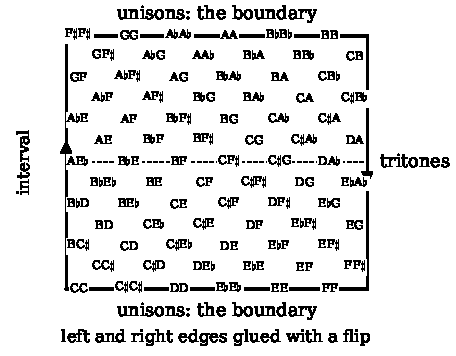
\includegraphics[width=0.55\textwidth,height=2.6in,keepaspectratio]{figs/app_dyads.pdf}\end{center}
An ordered pair of pitch classes is a point of $T^2=S^1\times S^1$. A two-note chord forgets the order, so the space of dyads is $T^2/S_2$, the quotient by swapping coordinates. Tymoczko observed that this quotient is a Möbius band. Its boundary is the fixed set of the swap, the unisons; the tritones, which divide the octave evenly, lie on the central circle. A voice leading from one dyad to another is a path, and its size is the length of the path. Moving across the band and out the side brings you back with the voices exchanged, which is the half-twist.
\begin{list}{}{\leftmargin=1.2em\itemindent=-1.2em\itemsep=0pt}\small \item D. Tymoczko, The geometry of musical chords, Science 313 (2006) 72.\end{list}
\subsection{Chord spaces as orbifolds}\label{app:app-orbifold}
\noindent\textit{Spaces:} n-torus (\S\ref{sp:ntorus}), Möbius band (\S\ref{sp:mobius}).\enspace\textit{Invariant:} $T^n/S_n$.

For $n$-note chords, ordered pitch-class tuples form $T^n$ and unordered chords form the orbifold $T^n/S_n$. For three notes this is a triangular prism whose two ends are glued with a third of a turn. The augmented triad, which divides the octave into three equal parts, lies on the central axis; major and minor triads lie close to it, and chords with repeated notes lie on the mirror boundary. Efficient voice leading is motion along short paths, and chords near the center can reach many other chords by short paths. This gives a geometric reason that nearly even chords such as triads and seventh chords support smooth voice leading. Callender, Quinn, and Tymoczko extended the picture to a family of quotient spaces obtained by imposing octave, permutation, transposition, inversion, and cardinality equivalences.
\begin{list}{}{\leftmargin=1.2em\itemindent=-1.2em\itemsep=0pt}\small \item D. Tymoczko, The geometry of musical chords, Science 313 (2006) 72.\item C. Callender, I. Quinn, D. Tymoczko, Generalized voice-leading spaces, Science 320 (2008) 346.\item D. Tymoczko, A Geometry of Music, Oxford University Press, 2011.\end{list}
\subsection{The Tonnetz is a torus}\label{app:app-tonnetz}
\noindent\textit{Spaces:} Torus (\S\ref{sp:torus}).\enspace\textit{Invariant:} $\mathbb{Z}^2/\Lambda\ \text{with}\ \Lambda\ \text{of index }12$.

\begin{center}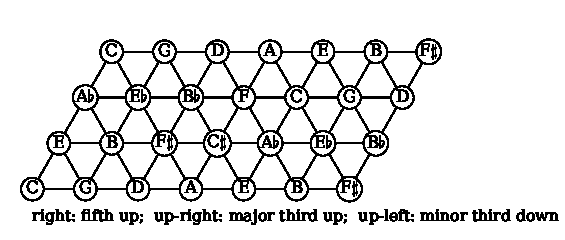
\includegraphics[width=0.55\textwidth,height=2.6in,keepaspectratio]{figs/app_tonnetz.pdf}\end{center}
Euler's Tonnetz arranges notes in a plane so that one direction moves by perfect fifths and another by major thirds; the third direction then moves by minor thirds. Major and minor triads are the triangles. In twelve-tone equal temperament, three major thirds return to the starting note and so do twelve fifths, so the plane is periodic in two independent directions and wraps into a torus. Neo-Riemannian theory studies the three operations that flip a triangle across one of its edges, keeping two notes and moving the third by a step. These flips generate chord progressions that move around the torus, common in late Romantic music and in film scores.
\begin{list}{}{\leftmargin=1.2em\itemindent=-1.2em\itemsep=0pt}\small \item R. Cohn, Introduction to neo-Riemannian theory: a survey and a historical perspective, Journal of Music Theory 42 (1998) 167.\end{list}
\subsection{Meter, polyrhythm, and phasing}\label{app:app-rhythm}
\noindent\textit{Spaces:} Circle (\S\ref{sp:circle}), Torus (\S\ref{sp:torus}), Dyadic solenoid (\S\ref{sp:solenoid}).\enspace\textit{Invariant:} $\text{lines of slope } p/q \text{ on } T^2$.

\begin{center}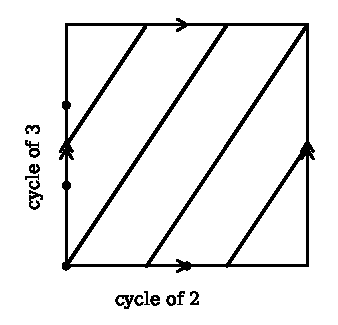
\includegraphics[width=0.55\textwidth,height=2.6in,keepaspectratio]{figs/app_poly.pdf}\end{center}
Cyclic meter puts time on a circle: a position in a bar is a point of $\mathbb{R}/\mathbb{Z}$. Two simultaneous cycles put time on a torus, and a $3{:}2$ polyrhythm is the closed line of slope $3/2$, with onsets where it crosses the edges of the square. If the two tempos drift apart slowly, as in Steve Reich's phasing pieces, the slope changes and the line moves across the torus; an irrational ratio of tempos would give a line that never closes and passes arbitrarily near every point. Iterated duple grouping (beat, bar, two-bar unit, four-bar unit) is a tower of circles each covering the next twice. The inverse limit of such a tower is the dyadic solenoid, with musical time running along a single path component. This last point is a modeling observation rather than an established result.
\begin{list}{}{\leftmargin=1.2em\itemindent=-1.2em\itemsep=0pt}\small \item S. Reich, Piano Phase (1967).\end{list}
\subsection{Topological analysis of recorded music}\label{app:app-musicdata}
\noindent\textit{Spaces:} Torus (\S\ref{sp:torus}), Circle (\S\ref{sp:circle}).\enspace\textit{Invariant:} $\text{persistent }H_1$.

Budney and Sethares applied persistent homology to features computed from recordings. Periodic structure in the sound shows up as persistent classes in degree one. In general, data governed by one cyclic parameter samples a circle, and data governed by two independent cyclic parameters samples a torus. The paper was among the most read in the Journal of Mathematics and Music, and it is a natural entry point for applying the data-analysis methods above to sound.
\begin{list}{}{\leftmargin=1.2em\itemindent=-1.2em\itemsep=0pt}\small \item R. Budney and W. Sethares, Topology of musical data, Journal of Mathematics and Music 8 (2014). \url{https://arxiv.org/abs/1307.1201}\end{list}
\section{Engineering and computation}
\subsection{Robot arms and motion planning}\label{app:app-robots}
\noindent\textit{Spaces:} n-torus (\S\ref{sp:ntorus}), Configuration space (\S\ref{sp:conf}), Finite connected graph (\S\ref{sp:graph}).\enspace\textit{Invariant:} $\text{continuous planner exists}\iff X\ \text{contractible}$.

A robot arm with $n$ rotating joints has configuration space $T^n$, one angle per joint. A motion planner is a rule that takes a start and an end configuration and returns a path between them. Farber showed that a planner depending continuously on its input exists only if the configuration space is contractible. Since $T^n$ is not, every planner for a jointed arm has discontinuities, and the minimal number of continuous pieces needed, the topological complexity, is a homotopy invariant. Configuration spaces of several robots moving on a network of tracks are configuration spaces of graphs, whose fundamental groups are braid groups of graphs.
\begin{list}{}{\leftmargin=1.2em\itemindent=-1.2em\itemsep=0pt}\small \item M. Farber, Topological complexity of motion planning, Discrete Comput. Geom. 29 (2003) 211.\item R. Ghrist, Configuration spaces and braid groups on graphs in robotics, AMS/IP Stud. Adv. Math. 24 (2001) 29.\end{list}
\subsection{Orientations, gimbal lock, and quaternions}\label{app:app-attitude}
\noindent\textit{Spaces:} Rotation group (\S\ref{sp:so3}), Sphere (\S\ref{sp:sphere}).\enspace\textit{Invariant:} $SO(3)\cong\mathbb{RP}^3$.

The orientation of a rigid body is a point of $SO(3)$, a compact 3-manifold. A compact 3-manifold cannot be covered by a single chart, so any description by three numbers, such as Euler angles, must break down somewhere; the breakdown is called gimbal lock. Stuelpnagel proved that no three-parameter representation is both global and nonsingular. Spacecraft attitude control and computer graphics therefore use unit quaternions, points of the double cover $S^3$, with $q$ and $-q$ representing the same rotation.
\begin{list}{}{\leftmargin=1.2em\itemindent=-1.2em\itemsep=0pt}\small \item J. Stuelpnagel, On the parametrization of the three-dimensional rotation group, SIAM Review 6 (1964) 422.\end{list}
\subsection{Kirchhoff's laws and the cycle space of a circuit}\label{app:app-kirchhoff}
\noindent\textit{Spaces:} Finite connected graph (\S\ref{sp:graph}), Wedge of n circles (\S\ref{sp:rose}).\enspace\textit{Invariant:} $\operatorname{rank}H_1(\Gamma)=E-V+1$.

An electrical network is a graph. Kirchhoff's voltage law requires one equation for each independent loop, and Kirchhoff showed that the number needed is $E-V+1$, which is the rank of $H_1$ of the graph. A spanning tree, the tool used in the graph entry to compute the fundamental group, picks out the independent loops: each edge outside the tree closes exactly one. This 1847 argument is among the earliest uses of what became homology.
\begin{list}{}{\leftmargin=1.2em\itemindent=-1.2em\itemsep=0pt}\small \item G. Kirchhoff, Über die Auflösung der Gleichungen, auf welche man bei der Untersuchung der linearen Vertheilung galvanischer Ströme geführt wird, Annalen der Physik 72 (1847) 497.\end{list}
\subsection{Observable properties and the Sierpiński space}\label{app:app-observable}
\noindent\textit{Spaces:} Sierpiński space (\S\ref{sp:sierpinski}), Countable cofinite space (\S\ref{sp:cofinite}).\enspace\textit{Invariant:} $\{\text{open sets of }X\}\leftrightarrow C(X,\mathbb{S})$.

In the semantics of programming languages, an open set is read as a property that can be confirmed by a finite amount of observation: a program halts, a stream contains a 1. Such properties can be verified but not always refuted, which is the asymmetry of the Sierpiński space, where $1$ is open and $0$ is not. A property of a space of computations is observable exactly when it is a continuous map to the Sierpiński space. The resulting topologies are $T_0$ but rarely $T_1$, so the non-Hausdorff entries of this zoo are the normal case in domain theory.
\begin{list}{}{\leftmargin=1.2em\itemindent=-1.2em\itemsep=0pt}\small \item S. Vickers, Topology via Logic, Cambridge University Press, 1989.\item M. B. Smyth, Power domains and predicate transformers: a topological view, ICALP 1983, LNCS 154.\end{list}
\subsection{Digital topology and finite spaces}\label{app:app-digital}
\noindent\textit{Spaces:} Pseudocircle (\S\ref{sp:pseudocircle}), Sierpiński space (\S\ref{sp:sierpinski}).\enspace\textit{Invariant:} $|K(X)|\to X\ \text{weak equivalence}$.

A digital image is a finite grid of pixels, and the question of which pixels form a connected region, or whether a closed curve of pixels separates the plane, depends on how neighbors are defined. Khalimsky, Kopperman, and Meyer gave the grid a finite $T_0$ topology in which pixels alternate between open and closed points, as in the pseudocircle, and in which a digital Jordan curve theorem holds. McCord's theorem, used in the pseudocircle entry, guarantees that such finite spaces can model the homotopy type of any finite simplicial complex.
\begin{list}{}{\leftmargin=1.2em\itemindent=-1.2em\itemsep=0pt}\small \item E. Khalimsky, R. Kopperman, P. R. Meyer, Computer graphics and connected topologies on finite ordered sets, Topology and its Applications 36 (1990) 1.\item M. C. McCord, Singular homology groups and homotopy groups of finite topological spaces, Duke Math. J. 33 (1966) 465.\end{list}
\subsection{The Zariski topology of a curve}\label{app:app-zariski}
\noindent\textit{Spaces:} Countable cofinite space (\S\ref{sp:cofinite}).\enspace\textit{Invariant:} $\text{closed sets}=\text{finite sets}$.

In algebraic geometry, the closed subsets of an irreducible algebraic curve are the zero sets of polynomials, which are the finite sets and the whole curve. So the Zariski topology on the points of a curve is the cofinite topology. It is compact and $T_1$ but not Hausdorff, exactly as in the countable cofinite entry, which is the curve's topology when its points are countable, as for a curve over the algebraic numbers. Much of the machinery of algebraic geometry, including sheaf cohomology, was built to do useful topology on spaces this coarse.
\begin{list}{}{\leftmargin=1.2em\itemindent=-1.2em\itemsep=0pt}\small \item R. Hartshorne, Algebraic Geometry, Springer, 1977, Chapter I.\end{list}
\section{Economics and everyday life}
\subsection{Nash equilibrium}\label{app:app-nash}
\noindent\textit{Spaces:} Closed disk (\S\ref{sp:disk}).\enspace\textit{Invariant:} $f:D^n\to D^n\ \Rightarrow\ \exists\,x=f(x)$.

In a finite game, a mixed strategy for each player is a probability vector, and the set of all strategy profiles is a product of simplices, homeomorphic to a closed disk. Nash defined a continuous map on this disk that moves each player's strategy toward better responses. Its fixed points are exactly the profiles where no player gains by changing strategy alone. Brouwer's theorem, proved in the disk entry with $H_{n-1}$, guarantees a fixed point, so every finite game has an equilibrium. The proof gives no way to find it, and computing Nash equilibria is believed to be hard in general.
\begin{list}{}{\leftmargin=1.2em\itemindent=-1.2em\itemsep=0pt}\small \item J. Nash, Non-cooperative games, Annals of Mathematics 54 (1951) 286.\end{list}
\subsection{The hairy ball theorem and the wind}\label{app:app-hairy}
\noindent\textit{Spaces:} Sphere (\S\ref{sp:sphere}), Torus (\S\ref{sp:torus}).\enspace\textit{Invariant:} $\chi(S^2)=2\ne0$.

A continuous tangent vector field on a closed surface has zeros whose indices add up to the Euler characteristic. Since $\chi(S^2)=2$, every continuous tangent field on a sphere vanishes somewhere. For an idealized continuous horizontal wind on the Earth's surface, there is always a point where the horizontal wind is zero, such as the eye of a cyclone. A torus has $\chi=0$ and carries nowhere-zero fields, which is one reason the torus entry and the sphere entry behave so differently.
\begin{list}{}{\leftmargin=1.2em\itemindent=-1.2em\itemsep=0pt}\small \item J. Milnor, Topology from the Differentiable Viewpoint, 1965, Chapter 6.\end{list}
\subsection{Borsuk–Ulam: antipodes and fair division}\label{app:app-borsuk}
\noindent\textit{Spaces:} Sphere (\S\ref{sp:sphere}), Real projective space (\S\ref{sp:rpn}).\enspace\textit{Invariant:} $f:S^n\to\mathbb{R}^n\ \Rightarrow\ \exists\,x:\ f(x)=f(-x)$.

The Borsuk–Ulam theorem says every continuous map $S^n\to\mathbb{R}^n$ sends some pair of antipodal points to the same value. With $n=2$: at any moment there are two antipodal points on the Earth with the same temperature and the same pressure. The proof passes to $\mathbb{RP}^n=S^n/\pm1$ and uses its mod 2 cohomology. The same theorem gives the ham sandwich theorem, that one plane cut can bisect three solids at once, and the necklace splitting theorem, that two thieves can fairly divide a necklace with $k$ kinds of beads using at most $k$ cuts.
\begin{list}{}{\leftmargin=1.2em\itemindent=-1.2em\itemsep=0pt}\small \item N. Alon, Splitting necklaces, Advances in Mathematics 63 (1987) 247.\item J. Matoušek, Using the Borsuk–Ulam Theorem, Springer, 2003.\end{list}
\chapter{Where computation gets hard}
\section{Homotopy groups of spheres}
Homology of $S^n$ vanishes above degree $n$, yet $\pi_k(S^n)$ is nonzero for infinitely many $k$ when $n\ge2$, and no closed formula is known.
\begin{center}\renewcommand{\arraystretch}{1.2}
\begin{tabular}{c|cccccccc}
 & $\pi_1$ & $\pi_2$ & $\pi_3$ & $\pi_4$ & $\pi_5$ & $\pi_6$ & $\pi_7$ & $\pi_8$\\\hline
$S^1$ & $\mathbb{Z}$ & $0$ & $0$ & $0$ & $0$ & $0$ & $0$ & $0$\\
$S^2$ & $0$ & $\mathbb{Z}$ & $\mathbb{Z}$ & $\mathbb{Z}_2$ & $\mathbb{Z}_2$ & $\mathbb{Z}_{12}$ & $\mathbb{Z}_2$ & $\mathbb{Z}_2$\\
$S^3$ & $0$ & $0$ & $\mathbb{Z}$ & $\mathbb{Z}_2$ & $\mathbb{Z}_2$ & $\mathbb{Z}_{12}$ & $\mathbb{Z}_2$ & $\mathbb{Z}_2$\\
$S^4$ & $0$ & $0$ & $0$ & $\mathbb{Z}$ & $\mathbb{Z}_2$ & $\mathbb{Z}_2$ & $\mathbb{Z}\oplus\mathbb{Z}_{12}$ & $\mathbb{Z}_2^2$\\
$S^5$ & $0$ & $0$ & $0$ & $0$ & $\mathbb{Z}$ & $\mathbb{Z}_2$ & $\mathbb{Z}_2$ & $\mathbb{Z}_{24}$
\end{tabular}\end{center}
\section{Undecidability}
Every finitely presented group is $\pi_1$ of a closed 4-manifold, and by the Adian--Rabin theorem no algorithm decides whether a finite presentation defines the trivial group. So no algorithm takes a triangulated 4-manifold and decides whether it is simply connected. In dimension 3, geometrization makes the word problem for fundamental groups solvable.
\section{Wild local behavior}
Van Kampen's theorem and covering space theory assume open sets that are path-connected and semilocally simply connected. The Hawaiian earring, the Warsaw circle, and the solenoid break these hypotheses, and their singular invariants stop agreeing with \v{C}ech invariants or with intuition.
\section{References}
A.~Hatcher, \emph{Algebraic Topology}, Cambridge, 2002 (free online). L.~A.~Steen and J.~A.~Seebach, Jr., \emph{Counterexamples in Topology}, 2nd ed., Springer-Verlag, New York, 1978; Dover reprint, 1995. The $\pi$-Base Community, S.~Clontz, and J.~Dabbs, $\pi$-Base, a community database of topological counterexamples, \url{https://topology.pi-base.org/}, data at \url{https://github.com/pi-base/data}, licensed CC BY 4.0. The Manifold Atlas, \texttt{map.mpim-bonn.mpg.de}. KnotInfo, \texttt{knotinfo.math.indiana.edu}.
\end{document}
